\documentclass[oneside,monografia]{iftex2020}

% --------------------------------------------------
% Pacotes
% --------------------------------------------------

\usepackage{varwidth}         % Legenda de figuras
\usepackage{fancyvrb}         % Ambiente mono-espaçado
\usepackage{fvextra}          % Melhorias no fancyvrb
\usepackage{textcomp}         % Símbulos extras
\usepackage{tabularx}         % Tabelas
\usepackage{csquotes}         % Citações

% Ajuste de espaçamento no Verbatim (fancyvrb)
\let\oldverbatim\Verbatim%
\let\oldendverbatim\endVerbatim%
\renewenvironment{Verbatim}%
  {\endgraf\vspace*{-1em}\oldverbatim}%
  {\oldendverbatim\vspace*{-1em}}%

% --------------------------------------------------
% Algoritmos
% --------------------------------------------------
\usepackage[noend]{algpseudocode}
% Comandos para traduzir as instruções do pacote de algoritmos
\algrenewcommand\algorithmicrequire{\textbf{Entrada:}}
\algrenewcommand\algorithmicensure{\textbf{Condição:}}
\algrenewcommand\algorithmicend{\textbf{fim}}
\algrenewcommand\algorithmicif{\textbf{se}}
\algrenewcommand\algorithmicthen{\textbf{então}}
\algrenewcommand\algorithmicelse{\textbf{senão}}
\algrenewcommand\algorithmicfor{\textbf{para}}
\algrenewcommand\algorithmicforall{\textbf{para todo}}
\algrenewcommand\algorithmicdo{\textbf{faça}}
\algrenewcommand\algorithmicwhile{\textbf{enquanto}}
\algrenewcommand\algorithmicrepeat{\textbf{repita}}
\algrenewcommand\algorithmicuntil{\textbf{até que}}
\renewcommand{\Return}{\State \textbf{retorne} }
\let\oldalgorithmic\algorithmic
\let\oldendalgorithmic\endalgorithmic
\renewenvironment{algorithmic}%
  {\hrulefill\vspace*{-0.5em}\oldalgorithmic}%
  {\oldendalgorithmic\vspace*{-1em}\hrulefill}

% --------------------------------------------------
% Comandos personalizados
% --------------------------------------------------
\newcommand{\comando}[1]{\textbf{$\backslash$#1}}
\newcommand{\ifmgtex}[1]{IFMG\TeX}


\addbibresource{referencias.bib}
% Na prática pode ser usado apenas \addbibresource{referencias.bib}
% O comando \addbibresource{referencias.bib} foi usado para mostrar as referências do capítulo de exemplo
% \addbibresource[label=bib:exemplo]{referencias_exemplos.bib}

% --------------------------------------------------
% Configurações do Documento
% --------------------------------------------------
\titulo{Desenvolvimento de um sistema para monitoramento de irrigação em tempo real}
\autor{Deivison Oliveira Costa}
\local{Bambuí - MG}
\data{07}{novembro}{2024}

% Instituição
\instituicao{IFMG}{Instituto Federal Minas Gerais}{Instituto Federal de Educação, Ciência e Tecnologia de Minas Gerais}
\unidade{\textit{Campus} Bambuí}
\curso{Bacharel}{Bacharelado}{Engenharia de Computação}

% Orientação
\orientador{Prof. Dr. Mateus Clemente de Sousa}

% Membros da banca examinadora (além do orientador e coorientador)
\membrobanca{Prof. Dr. Marcos Roberto Ribeiro}{IFMG -- \textit{Campus} Bambuí}
\membrobanca{Prof. Dr. Geraldo Henrique Alves Pereira}{IFMG -- \textit{Campus} Bambuí}

% -------------------------------------------------------
% Elementos Pré-textuais
% -------------------------------------------------------

% --------------------------------------------------
% Resumo e abstract (obrigatórios)
% --------------------------------------------------
\resumo{%
Este trabalho apresenta o desenvolvimento de um sistema de monitoramento em tempo real para a irrigação agrícola. O sistema integra tecnologias modernas, como Sistemas Cyberfísicos (CPS), aplicações web e protocolos de comunicação (HTTP e MQTT), com o método da Evapotranspiração da Cultura (ETc). A crescente demanda por soluções eficientes na gestão de recursos hídricos e a necessidade de práticas sustentáveis na agricultura motivam esta pesquisa. O sistema desenvolvido utiliza sensores de telemetria para coletar dados ambientais em tempo real. Além disso, algoritmos de cálculo da ETc são integrados ao sistema para fornecer métricas sobre as necessidades hídricas das culturas. A agricultura de precisão, aliada ao conceito de Internet das Coisas (IoT), permitem um monitoramento contínuo e detalhado das condições do solo e das plantas, promovendo uma gestão mais eficaz da irrigação. Espera-se que o sistema proposto contribua para a redução do desperdício de água, aumento da produtividade agrícola e promoção da sustentabilidade. Testes e validações em campo visam demonstrar a eficácia do sistema em fornecer informações úteis para os agricultores, facilitando a tomada de decisões.
}
\palavraschave{Monitoramento em tempo real. Agricultura de precisão. Evapotranspiração da Cultura (ETc). Protocolo MQTT. Internet das Coisas (IoT).}


% --------------------------------------------------
% Keywords e abstract
% --------------------------------------------------
\abstract{%
This work presents the development of a real-time monitoring system for agricultural irrigation. The system integrates modern technologies such as Cyber-Physical Systems (CPS), web applications, and communication protocols (HTTP and MQTT) with the Crop Evapotranspiration (ETc) method. The increasing demand for efficient water resource management solutions and the need for sustainable agricultural practices motivate this research. The developed system uses telemetry sensors to collect real-time environmental data. Additionally, ETc calculation algorithms are integrated into the system to provide metrics on crop water requirements. Precision agriculture, combined with the concept of the Internet of Things (IoT), allows for continuous and detailed monitoring of soil and plant conditions, promoting more effective irrigation management. It is expected that the proposed system will contribute to reducing water waste, increasing agricultural productivity, and promoting sustainability. Field tests and validations aim to demonstrate the system's effectiveness in providing useful information to farmers, facilitating decision-making.
}
\keywords{Real-time monitoring. Precision agriculture. Crop Evapotranspiration (ETc). MQTT protocol. Internet of Things (IoT).}

% Dedicatória (opcional)
\textodedicatoria{%
Dedico este trabalho a todos aqueles que acreditaram em mim. À minha família, pelo apoio e incentivo ao longo desta trajetória. Às minhas amizades, pelas palavras de encorajamento e momentos de descontração que me ajudaram a manter o equilíbrio. A todos que, de alguma forma, contribuíram para a minha formação acadêmica e pessoal, o meu mais sincero agradecimento.
}

% Agradecimentos (opcional)
\textoagradecimentos{%
Primeiramente, agradeço a Deus por guiar meus passos e iluminar meu caminho ao longo desta caminhada acadêmica. Sem sua orientação, nada disso seria possível. Agradeço por cada desafio superado, por cada aprendizado e por cada conquista.

Expresso minha gratidão ao meu orientador, Prof. Dr. Mateus, pela orientação produtiva, pelos conselhos e pela paciência dedicada na condução deste trabalho. Suas contribuições foram fundamentais para o meu crescimento acadêmico e profissional.

Agradeço também aos professores e colaboradores desta instituição, que compartilharam seus conhecimentos e experiências, enriquecendo meu percurso acadêmico e contribuindo para o desenvolvimento deste trabalho.

Aos meus pais e familiares, expresso minha profunda gratidão pelo apoio e pela compreensão durante todo este período. Vocês foram minha âncora nos momentos difíceis e minha maior fonte de inspiração.

Por fim, dedico um agradecimento especial aos meus amigos e colegas de estudo pela amizade e pela colaboração mútua. O apoio de vocês foi essencial.
}

% Epígrafe (opcional)
\textoepigrafe{%
    ``Bem-aventurado o homem que acha sabedoria, e o homem que produz conhecimento.''\\
    (Provérbios 3:13 - Bíblia Sagrada)
}

\listasiglas{%
 \begin{description}[leftmargin=3cm, labelindent=0cm]
    \item[ADC] -- Conversor Analógico-Digital (\textit{Analog-to-Digital Converter})
    \item[API] -- Interface de Programação de Aplicações (\textit{Application Programming Interface})
    \item[BDA] -- Análise de grandes dados (\textit{Big Data Analytics})
    \item[BLE] -- Bluetooth de Baixa Energia (\textit{Bluetooth Low Energy})
    \item[CERN] -- Organização Europeia para a Pesquisa Nuclear (\textit{Conseil Européen pour la Recherche Nucléaire})
    \item[CPU] -- Unidade Central de Processamento (\textit{Central Processing Unit})
    \item[CPS] -- Sistemas Ciberfísicos (\textit{Cyber-Physical Systems})
    \item[DDD] -- \textit{Design} Orientado a Domínio (\textit{Domain-Driven Design})
    \item[DIP] -- Princípio de Inversão de Dependência (\textit{Dependency Inversion Principle})
    \item[ETc] -- Evapotranspiração da Cultura
    \item[ETo] -- Evapotranspiração de Referência
    \item[GPIO] -- Pinos de Entrada/Saída Gerais (\textit{General-Purpose Input/Output})
    \item[HTML] -- Linguagem de Marcação de Hipertexto (\textit{HyperText Markup Language})
    \item[HTTP] -- Protocolo de Transferência de Hipertexto (\textit{Hypertext Transfer Protocol})
    \item[IA] -- Inteligência Artificial
    \item[IBM] -- International Business Machines
    \item[I2C] -- Circuito Inter-Integrado (\textit{Inter-Integrated Circuit})
    \item[IDE] -- Ambiente de Desenvolvimento Integrado (\textit{Integrated Development Environment})
    \item[INMET] -- Instituto Nacional de Meteorologia 
    \item[IoT] -- Internet das Coisas (\textit{Internet of Things})
    \item[IP] -- Protocolo de Internet (\textit{Internet Protocol})
    \item[ISP] -- Princípio de Segregação de Interface (\textit{Interface Segregation Principle})
    \item[JSON] -- Notação de Objetos JavaScript (\textit{JavaScript Object Notation})
    \item[Kc] -- Coeficiente de cultura
    \item[LAI] -- Índice de Área Foliar (\textit{Leaf Area Index})
    \item[LSP] -- Princípio de Substituição de Liskov (\textit{Liskov Substitution Principle})
    \item[MQTT] -- Protocolo de Telemetria de Fila de Mensagens (\textit{Message Queuing Telemetry Transport})
    \item[MVC] -- Modelo-Visão-Controle (\textit{Model-View-Controller})
    \item[OGC] -- Consórcio Geoespacial Aberto (\textit{Open Geospatial Consortium})
    \item[OCP] -- Princípio de Aberto/Fechado (\textit{Open/Closed Principle})
    \item[OPeNDAP] -- Projeto de código aberto para um protocolo de acesso a dados de rede (\textit{Open-source Project for a Network Data Access Protocol})
    \item[ORM] -- Mapeador Objeto-Relacional (\textit{Object-Relational Mapping}) 
    \item[PCB] -- Placa de Circuito Impresso (\textit{Printed Circuit Board})
    \item[QoS] -- Qualidade de Serviço (\textit{Quality of Service})
    \item[RAM] -- Memória de Acesso Aleatório (\textit{Random Access Memory})
    \item[ROM] -- Memória Somente de Leitura (\textit{Read-Only Memory})
    \item[SCPS] -- Sistemas Socio-Ciberfísicos (\textit{Social-Cyber-Physical Systems})
    \item[SI] -- Sistema Internacional de Unidades
    \item[SPI] -- Interface Periférica Serial (\textit{Serial Peripheral Interface})
    \item[SRP] -- Princípio de Responsabilidade Única (\textit{Single Responsibility Principle})
    \item[TCP] -- Protocolo de Controle de Transmissão (\textit{Transmission Control Protocol})
    \item[TLS] -- Segurança de Transporte de Camada (\textit{Transport Layer Security})
    \item[UART] -- Transmissor/Receptor Assíncrono Universal (\textit{Universal Asynchronous Receiver-Transmitter})
    \item[URI] -- Identificador Uniforme de Recurso (\textit{Uniform Resource Identifier})
    \item[USGS] -- Serviço Geológico dos Estados Unidos (\textit{United States Geological Survey})
    \item[WWW] -- Rede Mundial de Computadores (\textit{World Wide Web})
    \item[XML] -- Linguagem de Marcação Extensível (\textit{eXtensible Markup Language})
 \end{description}
}

\listasimbolos{%
  \begin{description}[leftmargin=3cm, labelindent=0cm]
    \item[$\Delta$] -- Déficit de pressão de vapor
    \item[$d_r$] -- Distância relativa inversa Terra-Sol
    \item[$e_a$] -- Pressão de vapor real
    \item[$e_s$] -- Pressão de vapor saturado
    \item[$E$] -- Irradiância solar
    \item[$ET_c$] -- Evapotranspiração da Cultura
    \item[$ET_o$] -- Evapotranspiração de Referência
    \item[$G$] -- Fluxo de calor no solo
    \item[$G_{sc}$] -- Constante solar (\(0.0820 \, MJ \, m^{-2} \, min^{-1}\))
    \item[$h$] -- Umidade do solo
    \item[$J$] -- Dia do ano 
    \item[$K_c$] -- Coeficiente de cultura
    \item[$lx$] -- Lux 
    \item[$P$] -- Pressão atmosférica 
    \item[$R^2$] -- Coeficiente de determinação
    \item[$R_a$] -- Radiação extraterrestre
    \item[$R_n$] -- Radiação líquida
    \item[$R_s$] -- Radiação solar
    \item[$R_{ns}$] -- Radiação solar líquida
    \item[$R_{nl}$] -- Radiação líquida de ondas longas
    \item[$R_{so}$] -- Radiação solar com céu limpo
    \item[$RH$] -- Umidade relativa do ar
    \item[$T$] -- Temperatura
    \item[$T_{max,K}$] -- Temperatura máxima em Kelvin
    \item[$T_{min,K}$] -- Temperatura mínima em Kelvin
    \item[$u_2$] -- Velocidade do vento a 2 metros de altura
    \item[$z$] -- Elevação em metros do nível do mar
    \item[$\delta$] -- Declinação solar 
    \item[$\gamma$] -- Constante psicrométrica
    \item[$\phi$] -- Latitude
    \item[$\omega_1$] -- Ângulo da hora solar no início do período 
    \item[$\omega_2$] -- Ângulo da hora solar no final do período 
    \item[$\sigma$] -- Constante de Stefan-Boltzmann (\(4.903 \cdot 10^{-9} \, MJ \, K^{-4} \, m^{-2} \, dia^{-1}\))
  \end{description}
}

% Ficha catalográfica (obrigatória)
%\ficha{ficha_catalografica}

% --------------------------------------------------
% Folha de aprovação (obrigatória)
% --------------------------------------------------
% Assinaturas e QRCode recortados do documento SEI
\assinaturas{assinaturas}

% -------------------------------------------------------
% Elementos opcionais
% -------------------------------------------------------

% Lista de figuras (opcional)
\listafiguras
% Lista de quadros (opcional)
%\listaquadros
% Lista de tabelas (opcional)
\listatabelas
% Lista de algoritmos (opcional)
%\listaalgoritmos
% Lista de códigos (opcional)
%\listacodigos

\begin{document}

% -------------------------------------------------------
% Gera elementos pré-textuais
% -------------------------------------------------------
\maketitle

% -------------------------------------------------------
% Capítulo: Introdução
% -------------------------------------------------------
\chapter{Introdução}

Na presente seção será apresentada uma contextualização do tema, posteriormente a justificativa e objetivos. Por fim, a estrutura do trabalho é mostrada.

\section{Contextualização do tema}
A agricultura é uma atividade fundamental para a economia global, sendo responsável pela produção de alimentos e matérias-primas essenciais para a sobrevivência e o bem-estar da humanidade. De acordo \textcite{carmody_fao2023}, o setor agrícola enfrenta desafios significativos. A crescente demanda por alimentos devido ao aumento populacional e as mudanças climáticas afetam a disponibilidade de recursos naturais. Diante desses desafios, a gestão eficiente dos recursos hídricos e a adoção de tecnologias avançadas tornam-se cruciais para garantir a sustentabilidade e a produtividade das culturas \parencite{carmody_fao2023}.

No Brasil, a agricultura desempenha um papel vital na economia, sendo uma das principais fontes de crescimento e desenvolvimento do país \parencite{Ramos_irrigacao2022}. O Brasil é um dos maiores produtores e exportadores de alimentos do mundo, destacando-se na produção de soja, milho, café e carne bovina \parencite{Ramos_irrigacao2022}. 

A irrigação é uma prática que tem sido objeto de estudo no país, visando aumentar a produtividade agrícola e contribuir para a segurança alimentar, conforme aponta \textcite{Ramos_irrigacao2022}. Métodos tradicionais de irrigação muitas vezes carecem de precisão e eficiência, levando ao desperdício de água e outros recursos \parencite{Pereira_irrigation2002}.

A evapotranspiração (ET) é uma das principais variáveis a serem consideradas na gestão eficiente da água \parencite{yang_nature2023}, sendo fundamental para determinar as necessidades hídricas das culturas e otimizar o uso da água na agricultura \parencite{carmody_fao2023, yang_nature2023}. Esta variável (ET) representa a perda de água do solo por evaporação e pela transpiração das plantas. 

O desenvolvimento de sistemas de monitoramento em tempo real para a irrigação surge como uma abordagem promissora para otimizar o uso da água e melhorar o rendimento das culturas \parencite{Vijh_system2024, Dutta_system2024, Amine_system2024}. De acordo com \textcite{Prathibha_system2017}, tais sistemas fornecem aos agricultores informações precisas e atualizadas sobre as condições do solo e das plantas, permitindo uma gestão mais eficiente da irrigação ao longo do tempo.

\section{Justificativa}

Este trabalho propõe o desenvolvimento de um sistema \textit{web} para monitoramento de variáveis ambientais, com o objetivo de otimizar a gestão da irrigação na agricultura. Integrando tecnologias de \textit{hardware} e \textit{software}, o sistema coleta e analisa dados climáticos em tempo real, oferecendo informações para a tomada de decisões mais sustentáveis e eficientes.

A adoção de ferramentas tecnológicas para o monitoramento ambiental incentiva a agricultura inteligente \parencite{Garg_smart2023}. Essas tecnologias permitem o ajuste dinâmico das atividades agrícolas com base nas variáveis climáticas coletadas. Isso possibilita aos produtores maximizar a produtividade enquanto reduzem os impactos ambientais, especialmente no uso de água \parencite{Gurjeet_smart2022}.

Considerando o alto consumo hídrico da agricultura, são necessárias soluções para otimizar o uso desses recursos \parencite{Ramos_irrigacao2022}. Ferramentas de monitoramento mais precisas podem favorecer uma gestão hídrica eficiente, reduzindo o desperdício e os custos operacionais \parencite{carmody_fao2023}.

Assim, a relevância deste estudo está na contribuição para uma agricultura mais prática e adaptável, que responda às diferentes condições climáticas e de solo, promovendo um modelo de produção sustentável.

\section{Objetivos}

Este trabalho tem como objetivo geral desenvolver um sistema de monitoramento em tempo real para o cultivo agrícola. A proposta é utilizar tecnologias modernas, como Sistemas Cyberfísicos (CPS), aplicações web e protocolos de comunicação (HTTP e MQTT), com o método da Evapotranspiração da Cultura (ETc). O objetivo é aumentar a eficácia do monitoramento da cultura e de suas necessidades hídricas.

Os objetivos específicos deste trabalho são os seguintes:

\begin{itemize}
    \item Implementar um sistema de telemetria de sensores para coletar dados ambientais-chave em tempo real;
    \item Integrar algoritmos de cálculo da ETc ao sistema para fornecer métricas;
    \item Desenvolver uma interface de usuário intuitiva para facilitar o acesso e a compreensão dos dados pelos agricultores.
\end{itemize}

\section{Estrutura do trabalho}
Este trabalho está estruturado da seguinte forma:

\begin{itemize}
    \item O Capítulo 2 apresenta os conceitos e teorias que servem como base para o desenvolvimento deste trabalho, além de fornecer o estado da arte da área de estudo;
    \item O Capítulo 3 descreve os procedimentos, técnicas e ferramentas utilizadas para a condução do trabalho;
    \item O Capítulo 4 expõe os principais achados do estudo, analisando os dados obtidos e destacando suas implicações.
    \item O Capítulo 5 apresenta a conclusão do trabalho, discutindo os resultados obtidos e as contribuições do estudo.
    \item Por fim, o Capítulo 6 traz possíveis direções futuras para a continuidade e aprimoramento do sistema proposto.
\end{itemize}


\chapter{Fundamentação teórica}

A seguir, são apresentadas perspectivas teóricas relevantes para o contexto do presente
trabalho.
\section{Sensoriamento remoto}
O sensoriamento remoto é uma área fundamental em vários campos científicos e tecnológicos. Ele pode ser definido  como:
\begin{quote}
"A arte ou ciência de dizer algo sobre um objeto sem tocá-lo". \parencite[{p. 34}]{fischer1976}
\end{quote}

Ao longo dos anos, o sensoriamento remoto tem evoluído, proporcionando uma variedade de aplicações em diversas áreas. Uma visão geral da evolução do sensoriamento remoto pode ser observada na Tabela \ref{tab:evolucao_sr}

\begin{table}[!htb]
\caption{Evolução do sensoriamento remoto.} \label{tab:evolucao_sr}
\begin{tabularx}{\textwidth}{|c|X|} \hline
\textbf{Ano} & \textbf{Evento} \\ \hline
1800         & Descoberta do infravermelho por Sir William Herschel. \\ \hline
1839         & Início da prática da fotografia. \\ \hline
1847         & Espectro infravermelho mostrado por A. H. L. Fizeau e J. B. L. Foucault para compartilhar propriedades com a luz visível. \\ \hline
1850-1860    & Fotografia a partir de balões. \\ \hline
1873         & Teoria da energia eletromagnética desenvolvida por James Clerk Maxwell. \\ \hline
1909         & Fotografia a partir de aviões. \\ \hline
1914-1918    & Primeira Guerra Mundial: reconhecimento aéreo. \\ \hline
1920-1930    & Desenvolvimento e aplicações iniciais da fotografia aérea e fotogrametria. \\ \hline
1929-1939    & Depressão econômica gera crises ambientais que levam a aplicações governamentais da fotografia aérea. \\ \hline
1930-1940    & Desenvolvimento de radares na Alemanha, Estados Unidos e Reino Unido. \\ \hline
1939-1945    & Aplicações da Segunda Guerra Mundial de porções não visíveis do espectro eletromagnético. \\ \hline
1950-1960    & Pesquisa e desenvolvimento militares. \\ \hline
1956         & Pesquisa de Colwell sobre detecção de doenças de plantas com fotografia infravermelha. \\ \hline
1960-1970    & Primeiro uso do termo sensoriamento remoto, satélite meteorológico TIROS. \\ \hline
1972         & Lançamento do Landsat 1. \\ \hline
1970-1980    & Avanços rápidos no processamento digital de imagens. \\ \hline
1980-1990    & Landsat 4: nova geração de sensores Landsat. \\ \hline
1980s        & Desenvolvimento de sensores hiperespectrais. \\ \hline
1990s        & Sistemas globais de sensoriamento remoto, lidares. \\ \hline
2000s        & Lançamento dos satélites Terra e Aqua da NASA para monitoramento climático. \\ \hline
2010s        & Lançamento dos satélites Sentinel pelo programa Copernicus da ESA. \\ \hline
\end{tabularx}
\fonte{Retirado de \textcite{campbell2011}.}
\end{table}

Uma das áreas de aplicação do sensoriamento remoto na atualidade é a agricultura. Estudos recentes, como o de \textcite{weiss2020}, destacam sua importância na adaptação e evolução das práticas agrícolas. Eles fornecem informações repetitivas sobre o estado das culturas ao longo da safra, em diferentes escalas e para diferentes partes interessadas.

As pesquisas ressaltam suas vantagens na monitorização das culturas, estimativa de produtividade e tomada de decisão em diferentes estágios da produção agrícola \parencite{shanmugapriya2019, khanal2020}. Entre esses benefícios, destacam-se a capacidade de monitorar vastas extensões de terra de maneira rápida e eficaz, a obtenção de informações em tempo real e a habilidade de integrar dados oriundos de diversas fontes para análises mais abrangentes.

Além disso, estudos evidenciam seu papel na obtenção de estatísticas agrícolas, contribuindo para a definição de unidades amostrais, estratificação e alocação de amostras \parencite{carfagna2005}. Essa contribuição é viabilizada pela integração de análise de imagens de satélite e dados de sensores, permitindo estimar com precisão a área plantada e a produtividade das culturas. Isso fornece subsídios essenciais para a formulação de políticas públicas e embasamento na tomada de decisões estratégicas no âmbito agrícola.

\subsection{Telemetria}
A telemetria é um campo complementar ao sensoriamento remoto e é definida como:
\begin{quote}
"A indicação, registro ou integração de uma quantidade em um ponto remoto por meios eleitorais e de tradução métrica.  Grandezas de estados elétricos ou mecânicos estão normalmente envolvidas, embora existam outras aplicações diversas para telemedição". \parencite[{p. 3}]{telemetering1941}
\end{quote}

De acordo com \textcite{telemetry_systems2002}, ao longo das décadas, os sistemas de telemetria evoluíram gradativamente, impulsionados por avanços tecnológicos em eletrônica, comunicações e processamento de dados. Inicialmente, a telemetria era predominantemente utilizada em aplicações aeroespaciais e militares para monitorar o \textit{status} e o desempenho de aeronaves e foguetes. 

Com o passar do tempo, sua aplicabilidade se expandiu para uma variedade de setores, incluindo medicina, indústria automotiva, energia e telecomunicações \parencite{Lizhuang_telemetry2021, Hassanien2020, Ding_telemetry2017}.

Para \textcite{Lizhuang_telemetry2021}, os avanços na miniaturização de sensores e no aumento da capacidade de armazenamento de dados possibilitaram a coleta de uma quantidade crescente de dados de telemetria. Além disso, melhorias nas técnicas de transmissão de dados têm aprimorado a análise dessas informações. 

\textcite{Ding_telemetry2017} afirmam que o desenvolvimento de algoritmos de análise de dados e inteligência artificial (IA) tem permitido uma compreensão mais profunda dos padrões e tendências nos dados telemétricos. Isso tem levado a aprimoramentos em diversos processos e sistemas.

Neste trabalho, a telemetria é empregada para monitorar variáveis ambientais, tais como umidade do solo, temperatura e umidade relativa do ar, em uma área de cultivo.  Os dados são coletados por sensores remotos e transmitidos através de protocolos de comunicação. Os protocolos de comunicação usados neste projeto foram o Transporte de Telemetria de Enfileiramento de Mensagens - MQTT (sigla do inglês \textit{Message Queuing Telemetry Transport}) e o Protocolo de Transferência de Hipertexto - HTTP (sigla do inglês \textit{Hypertext Transfer Protocol}) para um servidor remoto (\textit{broker}).

\section{Sistemas embarcados}
Há várias concepções propostas para sistemas embarcados; um conceito geral pode ser definido como:

\begin{quote}
"Aquele que possui \textit{hardware} de computador com \textit{software} embutido como um de seus componentes mais importantes. É um sistema baseado em computador dedicado para uma ou várias aplicações. Pode ser um sistema independente ou parte de um sistema maior". \parencite[{p. 39}]{dutta2014comprehensive}
\end{quote}

Sua utilização abrange desde dispositivos simples, como controles remotos e eletrodomésticos, até sistemas complexos, como veículos autônomos e equipamentos médicos \parencite{lee2008cyber, kato2018autoware}. Eles desempenham um papel fundamental na automação de processos industriais, na monitoração e controle de dispositivos, na coleta e processamento de dados em tempo real, entre outras funções \parencite{dutta2014comprehensive}.

Os sistemas embarcados são compostos por diversos componentes, incluindo microcontroladores, sensores, atuadores, interfaces de comunicação e \textit{software} embarcado \parencite{lee2008cyber}.
Eles são projetados para atender a requisitos específicos de desempenho, consumo de energia, tamanho e custo, dependendo da aplicação \parencite{Mazid_microcontrolador2011}.

Na seção seguinte, serão abordados os microcontroladores e sua importância na implementação de soluções embarcadas.

\section{Microcontroladores}

Segundo \textcite{lee2008cyber}, os microcontroladores são componentes essenciais dos sistemas embarcados. Estes desempenham um papel central na execução de tarefas específicas e no controle de dispositivos em uma variedade de aplicações. São compostos por:

\begin{quote}
  "Um microprocessador (CPU), além de uma quantidade fixa de memória principal (RAM), memória de programa (ROM/Flash),  interfaces de entrada/saída (I/O), temporizadores e conversores analógico-digitais (ADC), todos em um único chip". \parencite[{p. 40}]{Mazid_microcontrolador2011}
\end{quote}

A Tabela \ref{tab:evolucao_microcontroladores} mostra alguns modelos de microcontroladores e suas finalidades, desde modelos antigos até os mais recentes. Neste trabalho, o principal motivo da escolha do microcontrolador ESP32 se deu em razão de sua capacidade de comunicação \textit{wireless} embutida. Esse recurso também é nativo em outros microcontroladores, como Raspberry Pi 4, porém, o ESP32 se destaca por um menor custo e consumo de energia \parencite{ESP32_usage}.

\begin{table}[!htb]
\caption{Evolução dos microcontroladores.} \label{tab:evolucao_microcontroladores}
\begin{tabularx}{\textwidth}{|c|c|c|X|} \hline
\textbf{Modelo} & \textbf{Ano de Lançamento} & \textbf{Preço (USD)} & \textbf{Componentes Embutidos} \\ \hline
Intel 8051 & 1977 & \$1 - \$2 & CPU de 8 bits, memórias RAM e ROM integradas, temporizador, portas de I/O \parencite{8051_usage}. \\ \hline
PIC16F84A & 1993 & \$2 - \$4 & CPU de 8 bits, memórias flash e RAM integradas, temporizador, portas I/O \parencite{PIC16F84A_usage}. \\ \hline
Arduino Uno & 2010 & \$3 - \$4 & CPU de 8 bits, memórias flash e RAM integradas, temporizador, portas I/O digitais, USB \parencite{Arduino_usage}. \\ \hline
STM32F4 & 2011 & \$20 - \$25 & CPU de 32 bits, memórias flash e RAM integradas, temporizador, interfaces SPI, UART, I2C \parencite{STM32F4_usage}. \\ \hline
ESP32 & 2016 & \$3 - \$4 & CPU de 32 bits, \textit{Wi-Fi} e \textit{Bluetooth} integrados, memórias flash e RAM integradas, temporizador, portas GPIO, SPI, UART, I2C \parencite{ESP32_usage}. \\ \hline
Raspberry Pi 4 & 2019 & \$55 - \$60 & CPU de 64 bits, memória RAM integrada, Ethernet, Wi-Fi, portas USB, HDMI, GPIO \parencite{RaspberryPi4_usage}. \\ \hline
\end{tabularx}
\fonte{Elaborado pelo autor, 2024.}
\end{table}

A seguir, serão discutidas as características do ESP32 e sua relevância  na implementação de sistemas de monitoramento e controle.

\subsection{ESP32}

O ESP32 é um microcontrolador de baixo custo desenvolvido pela Espressif Systems. De acordo com \textcite{ESP32_usage}, este componente é amplamente utilizado em projetos de Internet das Coisas - IoT (sigla do inglês \textit{Internet of Things}) -devido à sua capacidade de conexão integrada e poder de processamento.

Baseado em um microprocessador \textit{dual-core} Tensilica Xtensa LX6, o ESP32 opera em frequências de até 240 MHz, apresentando uma arquitetura de 32 bits. Além disso, possui uma variedade de periféricos (Tabela \ref{tab:esp32_perifericos}), o que o torna versátil para uma variedade de aplicações \parencite{EspressifESP32}.

Uma das principais vantagens do ESP32, como destacado por \textcite{ESP32_usage}, é sua capacidade de conexão Wi-Fi e Bluetooth embutida, suportando os padrões 802.11 b/g/n Wi-Fi, Bluetooth 4.2 e Bluetooth Low Energy (BLE). Isso possibilita a comunicação sem fio em ambientes de IoT.

O ESP32 pode ser programado usando-se o Arduino IDE e o ESP-IDF (Espressif IoT Development Framework), ambos baseados em C/C++. Por meio dessas plataformas (IDEs), os desenvolvedores podem acessar os recursos do ESP32 e criar aplicações. Esses projetos vão desde simples automações residenciais até dispositivos complexos de monitoramento \parencite{ferrandez2018precision, junior2022data, hsu2020creative}.

Neste trabalho, o ESP32 atua como um ponto de controle, permitindo a comunicação bidirecional entre o mundo físico (representado pelas variáveis ambientais) e o mundo digital (representado pelo \textit{broker}). Essa capacidade de interação direta entre \textit{hardware}, \textit{software} e o ambiente físico exemplifica a definição de um Sistema Cyberfísico - CPS (sigla do inglês \textit{Cyber-Physical System}), como será abordado na próxima subseção.

\begin{table}[!htb]
  \caption{Periféricos do microcontrolador ESP32} \label{tab:esp32_perifericos}
  \begin{tabularx}{\textwidth}{|c|X|X|} \hline
    \textbf{Abreviação} & \textbf{Significado} & \textbf{Função} \\ \hline
    GPIO & Entrada/saída de uso geral. & Permite a comunicação de propósito geral com dispositivos externos através de sinais de entrada e saída digitais.  \\ \hline
    UART & Receptor/transmissor assíncrono universal. & Facilita a comunicação serial assíncrona entre o microcontrolador e outros dispositivos, como sensores e módulos de comunicação. \\ \hline
    SPI & Interface periférica serial. & Permite a comunicação serial síncrona de alta velocidade entre o microcontrolador e dispositivos periféricos, como sensores, displays e memórias. \\ \hline
    I2C & Circuito Interintegrado. & Oferece uma interface serial de dois fios para comunicação entre vários dispositivos. \\ \hline
  \end{tabularx}
  \fonte{Adaptado de \textcite{EspressifESP32}.}
\end{table}

\section{Sistemas cyberfísicos}

Os sistemas CPSs representam uma evolução dos sistemas embarcados. Eles podem ser definidos como:

\begin{quote}
"Integrações de computação com processos físicos. Computadores embarcados e redes que monitoram e controlam os processos físicos, geralmente com \textit{loops} de \textit{feedback} onde os processos físicos afetam as computações e vice-versa". \parencite[{p. 363}]{lee2008cyber}
\end{quote}

Recentemente, tem havido uma tendência crescente no uso de CPSs em aplicações práticas na agricultura. Por exemplo, \textcite{ahmad2020smart} demonstraram um sistema de monitoramento inteligente que utiliza abordagens para rastrear o comportamento e as atividades de roedores no campo. O sistema auxilia especialistas e agricultores em controle de pragas na aplicação mais eficiente de métodos de controle tradicionais.

Da mesma forma, \textcite{rad2015smart} propuseram um modelo de arquitetura de CPS para o monitoramento de culturas de batata, resultando na melhoria da produtividade. \textcite{rijswijk2021digital} discutiram o papel dos sistemas sociocyberfísicos (SCPSs) na transformação digital da agricultura e das áreas rurais. Eles destacaram a necessidade de compreender as relações entre os aspectos sociais e tecnológicos para uma aplicação bem-sucedida.

O presente trabalho se enquadra na categoria de CPS, pois integra componentes físicos, computacionais e de comunicação. Seu papel é monitorar um processo físico (a irrigação) de maneira automatizada e em tempo real. A infraestrutura necessária para conectar dispositivos físicos à internet e entre si é definida como IoT, como será abordado na próxima subseção. 

\section{Internet das coisas}
A IoT é um campo multidisciplinar que se desenvolveu ao longo do tempo, com contribuições de diversas áreas. \textcite{datta2017} representa esse campo como um \textit{"tsunami"}, que começa com a exploração marítima, seguida pelo desenvolvimento da engenharia, passando pela automação, eletricidade, sensoriamento e culminando na IoT (Figura \ref{figura:evolucao_iot}). 

Cada uma dessas etapas representa um avanço na integração de tecnologia e comunicação, resultando em um sistema interconectado e inteligente. A exploração marítima marcou o início do uso de tecnologias para navegação e comunicação a longas distâncias. Com a engenharia, foram estabelecidas as bases para a construção de infraestruturas complexas e sistemas mecânicos. 

A automação trouxe a capacidade de controlar processos e máquinas de forma eficiente, enquanto os avanços na eletricidade permitiram a disseminação de dispositivos eletrônicos. O sensoriamento adicionou a capacidade de monitorar e coletar dados em tempo real, preparando o terreno para a IoT, onde todos esses elementos se unem para criar um ambiente altamente conectado e responsivo.

A IoT pode ser definida como:

\begin{quote}
"Um paradigma emergente de objetos cotidianos que, através da interação com o ambiente e com outros dispositivos, coletam e compartilham dados, geralmente utilizando protocolos de comunicação padronizados e interoperáveis, e, em alguns casos, interagindo com usuários ou outros dispositivos". \parencite[{p. 44}]{kortuem2009things}
\end{quote}

Segundo \textcite{minerva2015towards}, a ideia de IoT foi proposta pela primeira vez por \textcite{ashton1999things}. Ele argumentou que poderia revolucionar a maneira como se interage com o mundo físico, permitindo que artefatos se comuniquem entre si e com sistemas de computador.

Ao longo dos anos 2000, avanços em tecnologias de comunicação sem fio, sensores e sistemas embarcados possibilitaram o desenvolvimento prático da IoT, como destacado por \textcite{kortuem2009things}. Na década de 2010, a IoT começou a ganhar notoriedade em uma variedade de setores, incluindo saúde, manufatura, transporte e agricultura. Vários autores discutiram como essas tecnologias abriram caminho para a criação de redes de dispositivos interconectados em diversos campos \parencite{kortuem2009things, tan2010things, minerva2015towards}.

Atualmente, a IoT continua a evoluir, com o surgimento de novas tecnologias, como a computação em névoa, termo conhecido, em inglês, como \textit{fog computing}, e integrações com inteligências artificiais (IAs) \parencite{junior2022data}. Na agricultura, a IoT é empregada para melhorar a eficiência e produtividade.

O estudo conduzido por \textcite{ferrandez2018precision} exemplifica o uso da IoT para otimizar os processos agrícolas. Por meio de sensores interconectados, demonstrou-se ser possível monitorar uma série de variáveis físicas, como a umidade do solo, a temperatura e a umidade relativa do ar. Essa abordagem mostrou-se promissora, capacitando os agricultores a tomarem decisões mais embasadas em relação ao momento ideal para o plantio, à irrigação e à aplicação de fertilizantes.

Combinada à computação em névoa, a IoT possibilita o processamento local dos dados coletados pelos sensores, o que reduz o tempo de resposta e os custos associados ao envio e recebimento de dados \parencite{hsu2020creative}. Além disso, a integração com a IA permite a análise preditiva e a otimização desses sistemas, fornecendo informações que aumentam a produtividade e diminuem o desperdício.

Para facilitar a comunicação entre dispositivos, servidores e outros sistemas, o presente trabalho utilizou os protocolos HTTP e MQTT, os quais permitem o acesso remoto e o controle dos dispositivos conectados à IoT, como será abordado nas próximas subseções.

\begin{figure}[!htb] \centering
  \caption{\textit{"Tsunami"} da IoT} \label{figura:evolucao_iot}
  \begin{varwidth}{\linewidth}
    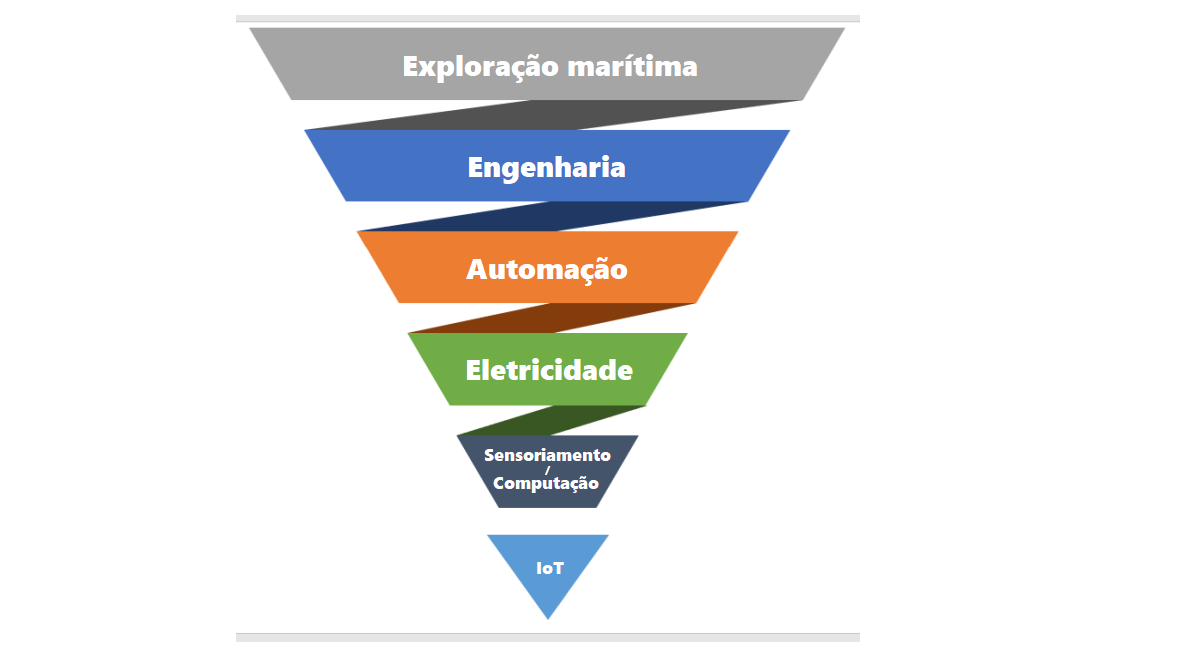
\includegraphics[width=16cm]{figuras/Datta.png}
    \fonte{Retirado de \textcite{datta2017}.}
  \end{varwidth}
\end{figure}

\section{Protocolo HTTP}
De acordo com \textcite{RFC2616}, o HTTP é um protocolo de comunicação utilizado para sistemas de informação distribuídos e colaborativos. Ele foi concebido para possibilitar a comunicação entre clientes e servidores na Rede Mundial de Computadores - WWW (sigla do inglês \textit{World Wide Web}).

O HTTP foi introduzido em 1989 por Tim Berners-Lee enquanto ele trabalhava na Organização Europeia para a Pesquisa Nuclear - CERN (sigla do francês \textit{Conseil Européen pour la Recherche Nucléaire}). A necessidade premente de compartilhar e distribuir informações de forma eficiente em uma rede de computadores motivou o desenvolvimento desse protocolo, que se tornou fundamental para a \textit{web} moderna \parencite{Berners_web}. Ele pode ser definido como:

\begin{quote}
"Um protocolo de camada de aplicação que define a estrutura de mensagens trocadas entre clientes e servidores. Ele opera sobre o Protocolo de Controle de Transmissão/Protocolo de Internet (TCP/IP), permitindo, nesta instância, a solicitação e transferência de recursos, como documentos HTML, imagens e vídeos, pela web". \parencite[{p. 7}]{RFC2616}
\end{quote}

No âmbito do desenvolvimento de sistemas, o HTTP desempenha um papel importante na criação de Interfaces de Programação de Aplicativos - APIs (sigla do inglês \textit{Application Programming Interfaces}), possibilitando a comunicação entre diferentes componentes. Os desenvolvedores têm a capacidade de criar pontos de acesso HTTP que aceitam solicitações e respondem com dados formatados, como JSON ou XML \parencite{Newmann_web}.

Na Tabela \ref{tab:metodos_http}, são destacados os principais métodos de solicitação do HTTP, utilizados para a interação entre clientes e servidores. No cotidiano, eles são usados para a obtenção de informações, o envio de dados e a execução de operações em sistemas distribuídos, como aplicações \textit{web} e APIs.

Contudo, por si só, o HTTP não é adequado para aplicações da IoT, devido à sua natureza orientada a texto e ao alto consumo de largura de banda \parencite{Yassein_mqtt2017}. Para esses casos, o protocolo MQTT é mais adequado, como será abordado na próxima subseção.

\begin{table}[!htb]
  \caption{Métodos HTTP} \label{tab:metodos_http}
  \begin{tabularx}{\textwidth}{|c|X|} \hline
    \textbf{Método} & \textbf{Descrição} \\ \hline
    GET & Solicita a representação de um recurso específico. \\ \hline
    POST & Envia dados para serem processados por um recurso identificado no servidor. \\ \hline
    PUT & Substitui todas as representações atuais do recurso de destino com os dados enviados na solicitação. \\ \hline
    DELETE & Remove o recurso identificado no URI. \\ \hline
    PATCH & Aplica modificações parciais a um recurso. \\ \hline  
  \end{tabularx}
  \fonte{Adaptado de \textcite{RFC2616}.}
\end{table}

\section{Protocolo MQTT}

O MQTT foi introduzido pela primeira vez em 1999 por Dr. Andy Stanford-Clark, da IBM, e Arlen Nipper, da Arcom (agora Eurotech) \parencite{Yassein_mqtt2017}. Segundo \textcite{Andy_mqtt2004}, o MQTT foi inicialmente desenvolvido para o monitoramento de oleodutos e gasodutos através de comunicações de telemetria. Ele é definido como:

\begin{quote}
"Um método de transporte de dados leve para publicação e assinatura sobre TCP/IP com várias garantias de entrega. Otimizado para uso mínimo de largura de banda de rede e facilidade de implementação em sistemas embarcados, ele serve como um mecanismo de transporte onde é possível decidir o que enviar e quais ações tomar ao receber os dados". \parencite[{p. 4}]{Andy_mqtt2004}
\end{quote}

Nos sistemas embarcados, o MQTT é implementado nos dispositivos para permitir a troca de dados \parencite{Andy_mqtt2004}. Os dispositivos podem publicar dados de sensores e \textit{status} usando tópicos MQTT, enquanto as aplicações podem se inscrever nesses tópicos para receber e processar os dados em tempo real \parencite{Yassein_mqtt2017}.

Do lado do servidor, os \textit{brokers} MQTT são implantados para gerenciar a troca de mensagens entre os dispositivos e as aplicações. Segundo \textcite{Yassein_mqtt2017}, esses \textit{brokers} são responsáveis por rotear as mensagens entre os clientes MQTT, garantindo a entrega dos dados. Além disso, os desenvolvedores podem usar bibliotecas MQTT em suas aplicações para se conectar aos \textit{brokers}, facilitando a implementação de funcionalidades de comunicação em seus sistemas \parencite{MQTT_org}.

Em sistemas IoT, o MQTT é utilizado para conectar dispositivos a plataformas de nuvem, permitindo o monitoramento e controle remoto dos dispositivos \parencite{junior2022data}. As aplicações podem processar os dados recebidos dos dispositivos IoT, realizar análises em tempo real e ações com base nos eventos detectados \parencite{ferrandez2018precision,hsu2020creative}. Suas principais características são definidas na Tabela \ref{tab:caract_mqtt}.

A implementação de sistemas de IoT na zona rural enfrenta desafios devido à baixa disponibilidade de internet e eletricidade, na maioria dos casos \parencite{rijswijk2021digital}. No entanto, o MQTT se destaca como uma solução para esses cenários. Ele oferece uma comunicação assíncrona entre dispositivos, reduzindo a dependência de conexões de alta velocidade e garantindo a entrega de mensagens \parencite{Andy_mqtt2004, Yassein_mqtt2017}. Essa característica o torna uma opção para superar limitações de infraestrutura em áreas remotas. 

Sua eficiência o posiciona como uma ferramenta para a agricultura inteligente \parencite{Gurjeet_smart2022}, tema que será discutido na próxima subseção.

\begin{table}[!htb]
  \caption{Características do protocolo MQTT} \label{tab:caract_mqtt}
  \begin{tabularx}{\textwidth}{|c|X|} \hline
    \textbf{Característica} & \textbf{Descrição} \\ \hline
    Leve & É leve e eficiente em termos de largura de banda e recursos de hardware. \\ \hline
    Assíncrono & Dispositivos podem enviar e receber mensagens de forma independente, sem bloqueio ou espera ativa. \\ \hline
    Padrão aberto & É um protocolo aberto e bem documentado. \\ \hline
    Qualidade de Serviço (QoS) & Oferece três níveis de QoS para garantir a entrega confiável das mensagens: QoS 0 (entrega no máximo uma vez), QoS 1 (entrega pelo menos uma vez) e QoS 2 (entrega exatamente uma vez). \\ \hline
    Tópicos & Usa um modelo de publicação/assinatura, onde os dispositivos podem publicar mensagens em tópicos específicos e se inscrever para receber mensagens de tópicos de interesse. \\ \hline  
    Baixa latência &  É projetado para minimizar a latência de rede, tornando-o adequado para casos de uso em tempo real, como telemetria, monitoramento e controle remoto. \\ \hline
    Segurança & Suporta autenticação e criptografia. \\ \hline
    Retenção de mensagens & Permite que o broker MQTT retenha as últimas mensagens publicadas em um tópico. \\ \hline  
  \end{tabularx}
  \fonte{Adaptado de \textcite{MQTT_org}.}
\end{table}

\section{Agricultura inteligente}
A agricultura passou por uma transformação impulsionada pelo advento das tecnologias digitais, marcando a era da agricultura inteligente. 

\begin{quote}
  "Também conhecida como agricultura 4.0 ou agricultura digital, é a próxima fase da agricultura industrial, impulsionada pela integração de tecnologias na agricultura". \parencite[{p. 424}]{Gurjeet_smart2022}
\end{quote}

Essa mudança de práticas agrícolas tradicionais para agricultura inteligente tornou-se imperativa. Ela é caracterizada pela integração de tecnologias emergentes, como a IoT, Análise de Dados em Grande Escala - BDA (siga do inglês \textit{Big Data Analysis}), computação em nuvem e IA. Seu objetivo é atender às crescentes demandas por segurança alimentar em uma população global em rápido crescimento \parencite{Gurjeet_smart2022, Garg_smart2023}.

Segundo \textcite{Garg_smart2023}, a convergência dessas tecnologias possibilitou o paradigma da agricultura orientada por dados, onde a coleta, análise e tomada de decisões em tempo real são centrais para otimizar práticas agrícolas.

\textcite{Gurjeet_smart2022} complementa que, ao elucidar o estado atual da adoção de tecnologia digital na agricultura e identificar perspectivas futuras, são abertos caminhos para práticas agrícolas sustentáveis e eficientes.

A agricultura inteligente, ao incorporar IA e análise avançada de dados, busca orientar decisões mais adaptativas e holísticas \parencite{Garg_smart2023}. Para isso, são necessárias a coleta e a aplicação precisa de dados para otimizar a produção \parencite{Lamine_precision2024}, o que será abordado na próxima subseção.

\section{Agricultura de precisão}

A agricultura de precisão pode ser definida como: 

\begin{quote}
  "A aplicação de tecnologias e princípios para gerenciar a variabilidade espacial e temporal associada a todos os aspectos da produção agrícola com o propósito de melhorar o desempenho das culturas e a qualidade ambiental". \parencite[{p. 1}]{Pierce_precision1999}
\end{quote}

Segundo \textcite{Pierce_precision1999}, o sucesso da agricultura de precisão está relacionado à sua capacidade de avaliar e gerenciar o continuum espaço-tempo na produção de culturas. Ela é habilitada pela tecnologia e integrada por tecnologias específicas que permitem avaliar e gerenciar a variabilidade em níveis de detalhe nunca antes alcançados \parencite{Zhang_precision2002}. No entanto, o sucesso agronômico da agricultura de precisão tem sido limitado e inconsistente, embora bastante convincente em alguns casos, complementa \textcite{Zhang_precision2002}.

Atualmente, de acordo com \textcite{Lamine_precision2024}, a agricultura de precisão é uma prática que busca observar, medir e responder às variações que ocorrem dentro de um mesmo campo e entre diferentes campos. Isso significa identificar as diferenças no solo, nas plantas e nas condições ambientais, tanto dentro de uma área de cultivo quanto entre áreas agrícolas distintas. Ao entender essas variações, é possível adotar abordagens específicas para cada local. Exemplo disso é ajustar a quantidade de fertilizantes ou de água, o que torna a produção mais eficiente e contribui para a conservação ambiental \parencite{Lamine_precision2024}.

Apesar dos avanços tecnológicos e inovações, a agricultura de precisão ainda enfrenta desafios em países em desenvolvimento, especialmente em agricultura de pequena escala, conforme apontado por \textcite{Lamine_precision2024}. No entanto, existem amplas oportunidades e perspectivas para a adoção de inovações em agricultura de precisão \parencite{Lamine_precision2024}.

A agricultura de precisão compreende um conjunto de tecnologias que combinam sensores e sistemas de informação. Essas tecnologias são utilizadas para otimizar a produção, levando em consideração a variabilidade e as incertezas dentro dos sistemas agrícolas. Ela fornece meios para monitorar a cadeia de produção de alimentos e gerenciar tanto a quantidade quanto a qualidade dos produtos agrícolas \parencite{Gebbers_precision2010}.

\textcite{Francisco_precision2024} demonstraram que a avaliação do ciclo de vida de tecnologias de agricultura de precisão possui potencial para melhorar a sustentabilidade agrícola, embora seu impacto ambiental exato permaneça incerto. Estudos comparativos mostraram que a agricultura de precisão pode reduzir os impactos ambientais da produção agrícola, especialmente no que diz respeito à gestão da irrigação \parencite{Francisco_precision2024}. No entanto, é importante considerar variáveis locais para uma avaliação ambiental abrangente, como será abordado na próxima subseção.

\section{Gestão da irrigação}

\textcite{Burton_irrigation2010} apresenta a gestão eficaz da irrigação como um desafio que demanda pesquisas e práticas sustentáveis, juntamente com o uso de tecnologias apropriadas. 
Considerando a complexidade das demandas e ofertas de recursos hídricos em perímetros irrigados, é essencial a utilização de técnicas e instrumentos para auxiliar profissionais nesse processo \parencite{Ramos_irrigacao2022}. Neste contexto, é fundamental o conhecimento da variabilidade espacial dos atributos do solo. Segundo \textcite{Ramos_irrigacao2022}, essa variabilidade está relacionada ao fluxo e armazenamento de água, usados como parâmetros para a otimização da produção agrícola.

\textcite{Pereira_irrigation2002} discutem diversos aspectos relacionados à gestão da irrigação em propriedades agrícolas, incluindo o uso de águas residuais tratadas e águas salinas. Os autores destacam a importância de estratégias como a uniformidade de distribuição e práticas de irrigação suplementar e deficitária para reduzir a necessidade de água na agricultura.

O estudo conduzido por \textcite{Burton_irrigation2010} complementa essas discussões. Ele destaca a importância das tecnologias, tais como o sensoriamento e a telemetria das condições ambientais, na agricultura irrigada. Além disso, ressalta a necessidade de desenvolver metodologias capazes de avaliar os benefícios sociais, econômicos e ambientais resultantes da otimização desse processo.

A integração dessas estratégias e tecnologias possibilita uma gestão mais eficiente da irrigação em áreas específicas, onde o consumo hídrico é variável \parencite{carmody_fao2023}. Essa integração, aliada à espacialização dos dados, apresentam melhorias efetivas no uso da água em escalas, como a de um perímetro irrigado \parencite{Burton_irrigation2010, Ramos_irrigacao2022}. Na próxima subseção, será discutida uma das perspectivas da gestão hídrica na agricultura, relevante para este trabalho.

\subsection{Gestão baseada no consumo de água}

Segundo \textcite{carmody_fao2023}, a gestão baseada no consumo de água traz uma perspectiva inovadora. Ela considera não apenas a entrega de água, mas também o uso real desta na agricultura. Isso contribui para a eficiência do uso dos recursos hídricos e para a sustentabilidade dos sistemas agrícolas. 

Na Figura \ref{figura:ciclo_agua}, é apresentado o ciclo da água. Ele é definido como um processo contínuo que envolve a precipitação, infiltração, evaporação, evapotranspiração (ET) e condensação \parencite{carmody_fao2023}. A água precipitada em forma de chuva ou neve alimenta os reservatórios superficiais e subterrâneos. Parte dela infiltra-se no solo, recarregando os lençóis freáticos, enquanto outra parte escoa superficialmente, mantendo o fluxo de rios e riachos. A evaporação dos corpos d'água e a ET das plantas retornam a umidade à atmosfera, onde se condensa formando nuvens, completando o ciclo.

Neste modelo, a água pode ser utilizada de duas formas: benéfica, como na transpiração das plantas para a produção de alimentos, e não benéfica, como na evaporação do solo nu ou de superfícies de água nuas. Também existem os fluxos de retorno não consumidos, que podem ser recuperados para consumo benéfico ou para manter os ecossistemas aquáticos (Figura \ref{figura:ciclo_agua}). Eles contribuem para o abastecimento de outros usuários a jusante e para a saúde dos rios e lençóis freáticos \parencite{carmody_fao2023}.

De acordo com \textcite{carmody_fao2023}, para alcançar economias reais de água, é necessário atender a quatro requisitos no contexto de um quadro mais amplo. Nesse quadro, os fluxos ambientais são considerados para sustentar os sistemas agrícolas e as pessoas que dependem deles. Esses requisitos incluem:

\begin{enumerate}
\item A determinação dos requisitos específicos de ET para a produção de culturas;
\item A definição dos direitos de água em termos de extração, consumo e fluxos de retorno;
\item O uso do monitoramento de ET e cobertura do solo para ajustar as alocações de água;
\item A comparação da ET alvo com a ET real para garantir um balanço hídrico adequado.
\end{enumerate}

Para compreender a ET e sua importância na gestão da água, é necessário analisar o cenário em que ela surge, como será abordado na próxima subseção.

\begin{figure}[!htb] \centering
  \caption{Ciclo Hidrológico} \label{figura:ciclo_agua}
  \begin{varwidth}{\linewidth}
    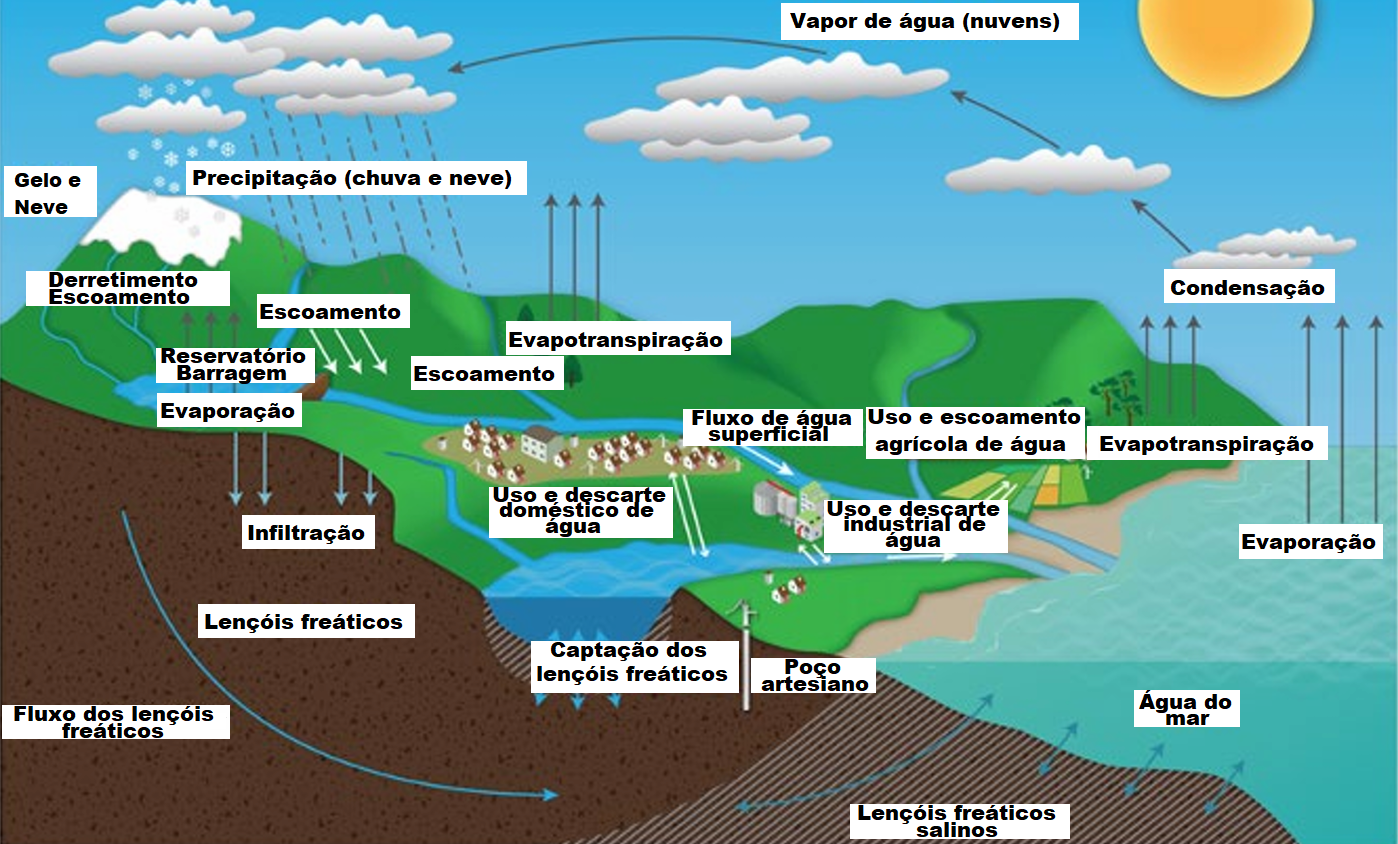
\includegraphics[width=16cm]{figuras/Carmody.png}
    \fonte{Retirado de \textcite{carmody_fao2023}.}
  \end{varwidth}
\end{figure}

\section{Evapotranspiração}

A ET descreve o processo fundamental de transferência de água da superfície da Terra para a atmosfera \parencite{carmody_fao2023}. Ela desempenha um papel importante na dinâmica hídrica. Foi observado que:

\begin{quote}
  "Três tipos de superfície são importantes no retorno da chuva à atmosfera. Para extensas áreas de terra, são eles, em ordem de importância: vegetação, na qual as folhas das plantas atuam como superfícies transpirantes; solo nu ou pousio, de onde a água evapora na interface solo-ar ou logo abaixo dela e em águas abertas, a partir das quais a evaporação ocorre diretamente". \parencite[{p. 121}]{Penman_evapotranspiration1948}
\end{quote}

\textcite{Penman_evapotranspiration1948} explica que a irrigação exerce influência direta na evaporação ao fornecer água ao solo. Esse processo não apenas afeta a disponibilidade de água para a evaporação, mas também influencia a temperatura e a umidade do solo, fatores determinantes para a taxa de ET. As interações entre a atividade humana e os ciclos naturais da água são particularmente relevantes no contexto das mudanças climáticas globais. 

Conforme destacado por \textcite{yang_nature2023}, tem-se observado uma tendência de aceleração no aumento da ET desde a década de 1980. Essa tendência está intimamente ligada à expansão da vegetação e ao aumento da área plantada, o que é evidenciado pelo crescimento do índice de área foliar (LAI).

O aumento da ET pode ter consequências tanto positivas quanto negativas. Por um lado, pode indicar um crescimento saudável da vegetação, o que pode ser benéfico para a agricultura e para a absorção de carbono. Por outro lado, um aumento excessivo da ET pode resultar em uma maior demanda por água, potencialmente levando ao estresse hídrico, especialmente em regiões onde a disponibilidade de água é limitada. \textcite{yang_nature2023} indicam a mensuração da ET para avaliar os impactos das atividades antropogênicas no ciclo hidrológico e no clima.

Métodos de telemetria da ET têm mostrado resultados promissores na compreensão desse fenômeno em escalas regional e global. De acordo com as revisões feitas por \textcite{Zhao_evapotranspiration_med2009, Zhang_evapotranspiration_med2016}, esses métodos variam desde modelos de equações simplificadas até modelos de balanço energético de duas fontes mais complexos. 

Segundo \textcite{Zhao_evapotranspiration_med2009}, os modelos mais eficazes utilizam sensores telemétricos que capturam a radiação emitida pelo solo, cobrindo desde o espectro visível até o infravermelho térmico. Essa abrangência espectral permite uma estimativa precisa da radiação líquida, um dos principais componentes do balanço de energia da superfície \parencite{Zhao_evapotranspiration_med2009}. No entanto, há uma dependência, em certa medida, de medições auxiliares baseadas em solo para derivar os fluxos de calor turbulentos em uma escala regional \parencite{Zhang_evapotranspiration_med2016}.

O coeficiente de determinação (\(R^2\)) é uma medida estatística que indica a proporção da variabilidade dos dados explicada pelo modelo \parencite{mood1974}. Ele é calculado pela fórmula:

\[
R^2 = 1 - \frac{\sum_{i=1}^n (y_i - \hat{y}_i)^2}{\sum_{i=1}^n (y_i - \bar{y})^2}
\]

\noindent em que: \(y_i\) são os valores observados, \(\hat{y}_i\) são os valores previstos pelo modelo, e \(\bar{y}\) é a média dos valores observados. O valor de \(R^2\) varia de 0 a 1, onde um valor próximo de 1 indica que o modelo explica a maior parte da variação nos dados. \textcite{Yang_evapotranspiration_med2022} apresenta um método de telemedição de ET com coeficiente de determinação de 0,88. Neste estudo, a fusão de dados de diferentes satélites (Landsat 8 e Sentinel-2), com resoluções espaciais e temporais variáveis, proporcionou uma estimativa contínua e precisa da ET diária em escala de campo.


Plataformas como o \textit{USGS EarthExplorer} e o \textit{Copernicus Open Access Hub} possuem acesso aberto às imagens dos satélites citados com alta resolução. Essas imagens serão utilizadas para a obtenção de dados no presente trabalho.

Nas duas próximas subseções, serão abordados conceitos e técnicas complementares às definições apresentadas acima, que foram de utilidade para o desenvolvimento do sistema proposto.

\subsection{Evapotranspiração de referência}

A ET de referência (ETo) é definida como:

\begin{quote}
  "A taxa de evapotranspiração de uma superfície de referência, sem falta de água". \parencite[{p. 7}]{Allen_evapotranspiration1998}
\end{quote}

Para calcular a ETo, pode-se empregar o método da FAO-56 apresentado por \textcite{Allen_evapotranspiration1998}, uma abordagem recomendada pela Organização das Nações Unidas para Alimentação e Agricultura, que é definida pela equação:

\begin{equation}
ETo = \frac{0.408 \cdot \Delta (R_n - G) + \gamma \cdot \frac{900}{T + 273} \cdot u2 \cdot (e_s - e_a)}{\Delta + \gamma \cdot (1 + 0.34 \cdot u2)}
\end{equation}

\noindent em que: ETo é a evapotranspiração de referência; $R_n$ é a radiação líquida; $G$ é o calor do solo; $\Delta$ é o déficit de pressão de vapor; $\gamma$ é a constante psicrométrica; $T$ é a temperatura média do ar; $u2$ é a velocidade do vento a 2 metros de altura; $e_s$ é a pressão de vapor do ar saturado; $e_a$ é a pressão de vapor do ar.

\subsection{Evapotranspiração de cultura}

A ET de cultura (ETc), por sua vez, é definida como:

\begin{quote}
  "A evapotranspiração de culturas livres de doenças, bem fertilizadas, cultivadas em grandes campos, sob condições ótimas de água no solo e atingindo plena produção nas condições climáticas dadas". \parencite[{p. 7}]{Allen_evapotranspiration1998}
\end{quote}

A ETc pode ser calculada como o produto da ETo e um determinado coeficiente de cultura (Kc), como proposto por \textcite{Allen_evapotranspiration1998}:

\begin{equation}
ETc = Kc \cdot ETo
\end{equation}

O Kc é um fator que leva em consideração as características específicas da cultura, como a fase de desenvolvimento, a densidade de plantio e a cobertura do solo. Ele é determinado experimentalmente e varia ao longo do ciclo de cultivo \parencite{bernardo_irrigacao2008}.

A determinação da ETc em tempo real é um dos principais objetos de estudo desta pesquisa. Na próxima seção, serão apresentados trabalhos similares e como a proposta deste trabalho se diferencia deles.

\section{Revisão bibliográfica}

O monitoramento da ETc é uma prática que possui diversas abordagens e métodos, dependendo do ambiente e do nível de precisão desejado. A ETc pode ser estimada por meio de métodos diretos, como a pesagem de lisímetros, ou indiretos, como a equação de \textcite{Allen_evapotranspiration1998}, apresentada na seção anterior. Entre essas abordagens, esta pesquisa propõe uma aplicação \textit{web} para o monitoramento da ETc em tempo real, combinando métodos indiretos para esse fim.

A seguir, serão apresentados outros trabalhos com abordagens semelhantes.

\subsection{Integração de dados e padrões \textit{web} para modelos de ETo}

\textcite{Jianting_webeva2009} abordam o desenvolvimento de sistemas de disseminação de dados em tempo real baseados na aquisição de dados. Eles fazem uso de dados geoespaciais para estimar a ETo diária, apontando a necessidade de métodos de acesso públicos a esses dados. Isso contrasta com os métodos utilizados nos serviços existentes com o mesmo propósito.

Os autores desenvolveram um sistema que utiliza padrões da \textit{Open Geospatial Consortium} (OGC) e o protocolo \textit{Network Data Access Protocol} (OPeNDAP) para publicar dados de estações meteorológicas. A arquitetura desse sistema incorpora diversas fontes de dados distribuídas e heterogêneas, como registros diários e horários de estações geoestacionárias. Além disso, imagens de satélite e resultados de modelos meteorológicos são utilizados para uma análise espacial. 

Por meio de serviços construídos sobre essas fontes, o sistema prova a eficácia de uma abordagem distribuída. Isso permite tanto a utilização quanto o desenvolvimento de novos serviços e aplicações sem interferir nos já existentes.

O trabalho de \textcite{Jianting_webeva2009} promove várias vantagens em relação à interoperabilidade e padronização de dados. No entanto, esse método não considera medições realizadas diretamente no local de interesse (\textit{in situ}). Isso, em cenários menores, como o de uma propriedade rural, pode ser uma limitação em questão de precisão e custo. Além disso, o sistema proposto não oferece uma interface para a visualização e análise dos dados, o que pode dificultar a interpretação dos resultados por usuários finais.

\subsection{Ferramentas \textit{web} para determinação de ETo}

O estudo de \textcite{Fangming_webeva2021} foca no desenvolvimento e implementação de APIs em nuvem, chamadas \textit{ETWatch}, para a geração de dados regionais da ETo. Essas APIs são desenvolvidas para proporcionar acesso fácil e em tempo real aos dados de ETo.

A metodologia combina dados de sensoriamento remoto, medições \textit{in situ} e modelagem matemática para calcular a evapotranspiração. As APIs facilitam a disseminação desses dados para diversos usuários e aplicações. Entre as vantagens do sistema \textit{ETWatch}, destacam-se o acesso em tempo real aos dados de ETo, permitindo uma resposta rápida para a gestão de recursos hídricos. Além disso, o sistema fornece uma interface para monitorar os dados, facilitando o acesso e a leitura das informações obtidas.

Apesar das vantagens, \textcite{Fangming_webeva2021} identificam alguns pontos que necessitam de maior preocupação. A precisão das estimativas pode ser limitada pela qualidade e disponibilidade dos dados de entrada, especialmente em regiões com poucas medições \textit{in situ}. A complexidade de integrar modelos climáticos e hidrológicos pode apresentar desafios computacionais e de implementação. Além disso, há a necessidade de ajustar os modelos para responder a variações e mudanças climáticas contínuas.

Uma abordagem semelhante foi realizada por \textcite{Jose_webeva2011} com o desenvolvimento de uma aplicação \textit{desktop} chamada \textit{CropWaterUse}. Essa aplicação foi desenvolvida para estimar os tempos de irrigação baseados na estimativa de ETc. Assim como \textcite{Fangming_webeva2021}, \textcite{Jose_webeva2011} utilizaram medições e modelos matemáticos para estimar a ETo. Contudo, eles realizaram o cálculo da ETc com base na ETo e em valores de Kc específicos para cada cultura, sendo estes inseridos manualmente pelo usuário na aplicação.

Porém, a aplicação \textit{CropWaterUse} não oferece uma interface de acesso distribuído para a visualização dos dados, seja por meio de APIs ou nuvens de dados. Isso limita sua utilização em cenários remotos ou até mesmo restritos, como propriedades rurais.

\subsection{Desenvolvimento e aplicação de ferramentas para ETo}
No estudo de \textcite{Taison_webeva2019}, foi desenvolvido um sistema que automatiza o cálculo da ETo, integrando dados de estações meteorológicas e métodos matemáticos. Diferentemente das pesquisas apresentadas, esse sistema adota o padrão de arquitetura \textit{Model-View-Controller} (\textit{MVC}) para o projeto. Esse \textit{design} separa a lógica de negócio, definida como \textit{Model}, da interface gráfica, chamada de \textit{View}. O \textit{Controller} é responsável por intermediar a comunicação entre o \textit{Model} e a \textit{View}. Dessa forma, é possível desacoplar as camadas do sistema, facilitando sua manutenção e evolução.

A aplicação de \textcite{Taison_webeva2019} é eficiente quanto à interface e à arquitetura. No entanto, o sistema não considera medições \textit{in situ} para o cálculo da ETo, o que pode limitar a precisão dos resultados para pequenas áreas, como já mencionado. 

Uma abordagem que contorna esse problema é apresentada por \textcite{Serban_webeva2022}. Ele destaca a criação e funcionalidade do \textit{ETCalc}, uma ferramenta gratuita para estimativa de ETo. Seu diferencial está na possibilidade de fornecer dados meteorológicos de múltiplas fontes. Ele permite que os usuários calculem a ETo em suas propriedades, com base em dados fornecidos de estações e medições locais. O \textit{ETCalc}, dentre as pesquisas encontradas, é a aplicação que possui o processamento matemático mais robusto, considerando diferentes métodos e parâmetros. Também fornece uma interface para a inserção e visualização dos dados, facilitando o acesso e o uso da ferramenta.

Apesar das vantagens, o \textit{ETCalc} falha como processo automatizado e em tempo real. O usuário precisa inserir manualmente os dados de entrada, o que pode ser um processo demorado e propenso a erros. Além disso, a ferramenta não oferece APIs para a integração com outros sistemas, o que limita sua utilização em cenários mais complexos.

Com base nas pesquisas apresentadas, na Tabela \ref{tab:comparacao}, é possível observar as tecnologias e métodos utilizados em cada uma delas. Também é possível identificar as limitações de cada abordagem, que servirão de base para o desenvolvimento da aplicação proposta nesta pesquisa.

\begin{table}[!htb]
    \caption{Comparação das tecnologias} \label{tab:comparacao}
    \begin{tabularx}{\textwidth}{|X|X|X|} \hline
        \textbf{Referência} & \textbf{Tecnologias} & \textbf{Limitações} \\ \hline
        \textcite{Taison_webeva2019} & \textit{PHP}, \textit{Smarty Template Engine}, \textit{HTML5}, \textit{CSS3}, \textit{JavaScript}, \textit{Bootstrap}, \textit{OpenLayers} e \textit{PostgreSQL}. & Escalabilidade limitada e performance inferior em aplicações complexas. \\ \hline
        \textcite{Serban_webeva2022} & \textit{Python}, \textit{Django}, \textit{HTML5}, \textit{CSS3}, \textit{JavaScript}, \textit{jQuery}, \textit{Bootstrap} e \textit{PostgreSQL}. & Menor performance em aplicações de alta carga e necessidade de alto conhecimento técnico em \textit{Python}. \\ \hline
        \textcite{Jose_webeva2011} & \textit{C\#}, \textit{ASP.Net}, \textit{Visual Studio.NET}, \textit{JavaScript}, \textit{TeeChart} e \textit{SQL Server}. & Dependência de plataforma \textit{Windows} e custos elevados de licenciamento. \\ \hline
        \textcite{Fangming_webeva2021} & \textit{Python}, \textit{Bootstrap}, \textit{jQuery}, \textit{Alibaba Cloud}, \textit{IDL}, \textit{Docker}, \textit{JSON} e \textit{PostgreSQL}. & Complexidade na integração e maior curva de aprendizado para configuração. \\ \hline
        \textcite{Jianting_webeva2009} & \textit{OGC standards}, \textit{OPeNDAP standards}, \textit{WMS}, \textit{WCS}, \textit{WFS}, \textit{GIS}, \textit{DODS}, \textit{DAS}, \textit{DDS} e \textit{Middleware components}. & Alta complexidade de implementação e necessidade de especialização em padrões \textit{OGC}. \\ \hline
        Presente pesquisa & \textit{C}, \textit{Node.js}, \textit{Next.js}, \textit{Shadcn/ui}, \textit{Tailwind CSS} e MQTT. & Alto consumo de memória em aplicações de alta carga e maior curva de aprendizado inicial para integração do MQTT. \\ \hline
    \end{tabularx}
    \fonte{Elaborado pelo autor, 2024.}
\end{table}


%  \chapter{Revisão bibliográfica}

%  \input{capitulos/cap_corpos_flutuantes}

\chapter{Materiais e métodos}

Nesta seção, são apresentados os materiais e métodos utilizados no desenvolvimento do sistema. Isso inclui as ferramentas e tecnologias empregadas, a arquitetura do sistema e as integrações realizadas.

\section{Descrição da área de estudo}
O sistema em questão foi implementado no Instituto Federal de Minas Gerais (IFMG), \textit{Campus} Bambuí, especificamente no Laboratório de Sistemas Embarcados. Esse local foi escolhido por possuir uma infraestrutura adequada para o teste de sensores e equipamentos necessários para a captura e transmissão de dados. A escolha do laboratório também se deve à disponibilidade de supervisão técnica e apoio logístico para a instalação e validação dos equipamentos.

\section{Classificação da pesquisa}

A pesquisa realizada no desenvolvimento do sistema de monitoramento meteorológico pode ser classificada segundo os seguintes critérios: quanto aos objetivos, à natureza, aos procedimentos técnicos e à abordagem do problema.

\subsection{Quanto aos objetivos}

De acordo com os objetivos, esta pesquisa é classificada como descritiva e exploratória. 

A pesquisa é descritiva porque visa descrever as características dos fenômenos meteorológicos monitorados pelos sensores, bem como o comportamento do sistema de monitoramento implementado. O foco foi detalhar como as variáveis meteorológicas, como temperatura, umidade, pressão, velocidade do vento e luminosidade, são capturadas e processadas pelo sistema, além de documentar o desempenho dos componentes de \textit{hardware} e \textit{software} utilizados.

A pesquisa também é exploratória porque busca investigar a aplicabilidade e eficiência de diferentes tecnologias e métodos no monitoramento meteorológico. Isso inclui a experimentação com diversos sensores e técnicas de integração de dados em um contexto específico. O caráter exploratório é acentuado pela busca de soluções tecnológicas que possam ser escaláveis e aplicáveis a diferentes contextos de monitoramento ambiental.

\subsection{Quanto à natureza}

Quanto à natureza, a pesquisa é aplicada. O objetivo principal foi o desenvolvimento de uma solução prática para um problema real, neste caso, a necessidade de monitoramento meteorológico em tempo real. O conhecimento gerado é voltado para a aplicação direta no sistema desenvolvido, com o propósito de melhorar a coleta, processamento e análise de dados meteorológicos. A pesquisa aplicada busca, portanto, transformar o conhecimento teórico em soluções práticas e funcionais.

\subsection{Quanto aos procedimentos técnicos}

Em relação aos procedimentos técnicos, a pesquisa é classificada como experimental. Durante o desenvolvimento do sistema, foram realizados testes e experimentos com diferentes componentes \textit{hardware} e \textit{software}, a fim de avaliar seu desempenho e adequação ao monitoramento meteorológico. Esses testes incluíram a validação dos sensores, a integração com o microcontrolador ESP32 e a transmissão de dados através do protocolo MQTT. A pesquisa experimental permitiu ajustes e refinamentos no sistema até alcançar um protótipo funcional e validado.

\subsection{Quanto à abordagem do problema}

Quanto à abordagem do problema, esta pesquisa é qualitativa. O sistema desenvolvido coleta, processa e fornece dados meteorológicos numéricos que são quantificados e apresentados em \textit{cards} interativos. Isso é feito por meio de uma interface de visualização com os dados capturados pelos sensores. Assim, foi possível a observação de variáveis como temperatura, umidade, pressão e velocidade do vento, além de possibilitar o cálculo de índices climáticos, como a evapotranspiração. A abordagem qualitativa foi escolhida como forma de interpretar os dados meteorológicos de maneira específica para cada área de coleta, permitindo uma análise detalhada das variáveis ambientais em seus contextos locais. Essa especificidade garante que os dados reflitam as condições e particularidades de cada região, favorecendo uma compreensão fundamentada dos fenômenos climáticos estudados.

\section{Componentes do Sistema de Monitoramento Meteorológico}

O sistema desenvolvido utiliza uma série de sensores para monitorar em tempo real diferentes parâmetros meteorológicos. Nesta seção, são apresentados os sensores e módulos utilizados no sistema, suas funcionalidades, características principais e como foram integrados ao microcontrolador ESP32 para a coleta e transmissão de dados meteorológicos.

\subsection{Sensor de Temperatura e Umidade DHT22}

O sensor DHT22 (Figura \ref{figura:dht22}) mede a temperatura e a umidade do ar, com precisão dentro do intervalo de operação \parencite{DHT22}. O pino de saída do sensor foi conectado ao pino GPIO 4 do ESP32, configurado no código como \texttt{DHTPIN}. Para alimentação, o sensor foi conectado ao pino 3V3 e ao GND do ESP32. Na Tabela \ref{tab:dht22}, são apresentadas as especificações técnicas do sensor.

O uso do sensor DHT22 no sistema justifica-se pela sua precisão dentro da faixa de operação desejada, característica necessária para o monitoramento climático \parencite{DHT22}. A medição precisa de temperatura e umidade relativa do ar é indispensável em aplicações meteorológicas, pois esses parâmetros influenciam diretamente fenômenos atmosféricos e condições ambientais. Além disso, a facilidade de integração ao ESP32 por meio de um único pino digital reduz a complexidade do circuito, otimizando a implementação do sistema. A escolha do DHT22, em detrimento de outros sensores, também considera o seu equilíbrio entre custo-benefício e desempenho, sendo utilizado em projetos de monitoramento ambiental \parencite{ferrandez2018precision,Francisco_precision2024}.

\begin{figure}[!htb] \centering
  \caption{Sensor de temperatura e umidade DHT22} \label{figura:dht22}
  \begin{varwidth}{\linewidth}
    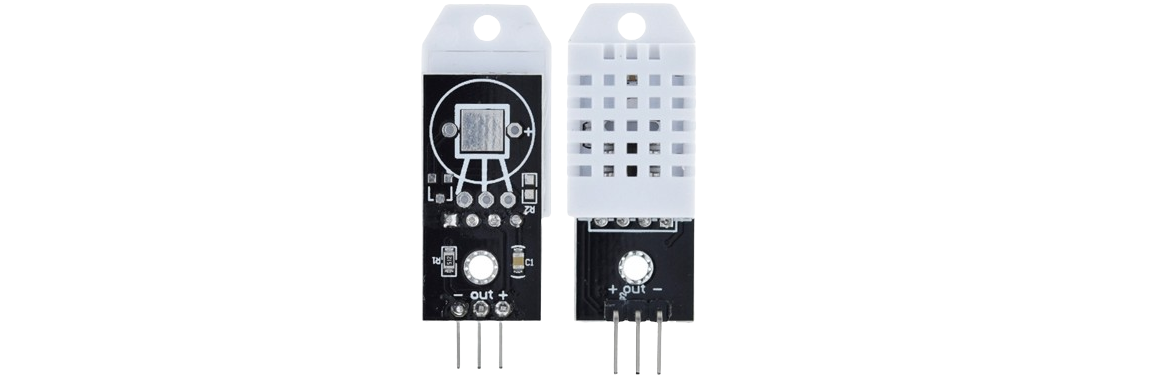
\includegraphics[width=16cm]{figuras/DHT22.png}
    \fonte{Retirado de \textcite{DHT22}.}
  \end{varwidth}
\end{figure}

\begin{table}[!htb]
    \caption{Especificações técnicas do sensor DHT22}
    \begin{tabularx}{\textwidth}{|X|X|} \hline
        \textbf{Parâmetro} & \textbf{Detalhes} \\ \hline
        Faixa de operação & Umidade: 0-100\% RH; Temperatura: -40\textdegree C a 80\textdegree C \\ \hline
        Precisão & Umidade: $\pm$2\% RH (Máx $\pm$5\%RH); Temperatura: $<$ $\pm$0.5\textdegree C \\ \hline
        Resolução/Sensibilidade & Umidade: 0.1\% RH; Temperatura: 0.1\textdegree C \\ \hline
        Período de amostragem & Média: 2 s \\ \hline
        Dimensões & 22x28x5 mm \\ \hline
    \end{tabularx}
    \label{tab:dht22}
    \fonte{Retirado de \textcite{DHT22}.}
\end{table}

\subsection{Sensor de Pressão BMP280}

O sensor BMP280 (Figura \ref{figura:bmp280}) mede a pressão atmosférica com precisão, além de oferecer medições de temperatura \parencite{BMP280}. Ele utiliza o barramento I2C, sendo conectado aos pinos padrão do ESP32 para \texttt{SDA} e \texttt{SCL}. Para alimentação, o sensor também foi conectado ao pino 3V3 e ao GND do ESP32. Na Tabela \ref{tab:bmp280}, são apresentadas as especificações técnicas do sensor.

A inclusão do sensor BMP280 no sistema deve-se à sua capacidade de medir pressão atmosférica com precisão, o que é necessário para a análise de condições meteorológicas e a previsão de mudanças climáticas \parencite{BMP280}. A pressão atmosférica é um parâmetro utilizado na modelagem de padrões climáticos, e o BMP280 oferece dados confiáveis dentro de uma faixa de operação desejada, adequado tanto para altitudes elevadas quanto para ambientes ao nível do mar. Além disso, a integração por barramento I2C simplifica a comunicação com o microcontrolador ESP32, permitindo o compartilhamento de pinos com outros dispositivos. A resolução do sensor possibilita a detecção de variações sutis na pressão, úteis para aplicações detalhadas, como estudos de microclimas \parencite{Prathibha_system2017, Lamine_precision2024}.

\begin{figure}[!htb] \centering
  \caption{Sensor de pressão barométrica BMP280} \label{figura:bmp280}
  \begin{varwidth}{\linewidth}
    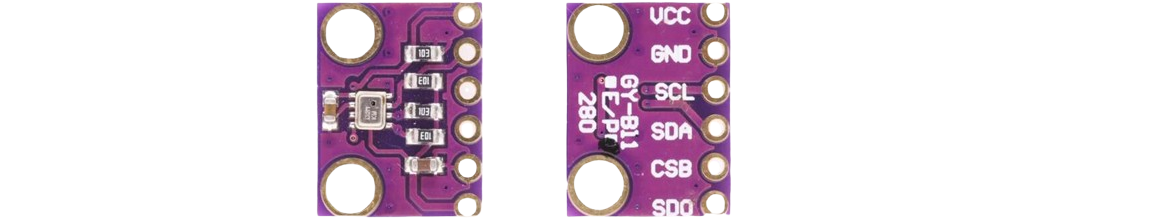
\includegraphics[width=16cm]{figuras/BMP280.png}
    \fonte{Retirado de \textcite{BMP280}.}
  \end{varwidth}
\end{figure}

\begin{table}[!htb]
  \caption{Especificações técnicas do sensor BMP280}
  \begin{tabularx}{\textwidth}{|X|X|} \hline
      \textbf{Parâmetro} & \textbf{Detalhes} \\ \hline
      Faixa de operação & 300-1100 hPa \\ \hline
      Precisão absoluta & $\sim$ $\pm$1 hPa (950-1050 hPa) \\ \hline
      Precisão relativa & $\pm$0.12 hPa (700-900 hPa) \\ \hline
      Resolução/Sensibilidade & 0.01 hPa (< 10 cm) \\ \hline
      Período de amostragem & Média: 5.5 ms \\ \hline
      Dimensões & 8x15.62x0.85 mm \\ \hline
  \end{tabularx}
  \label{tab:bmp280}
  \fonte{Retirado de \textcite{BMP280}.}
\end{table}

\subsection{Sensor de Luminosidade BH1750}

O BH1750 (Figura \ref{figura:bh1750}) é um sensor digital de luminosidade que mede a intensidade luminosa em lux. Ele também utiliza o barramento I2C, compartilhando os mesmos pinos do BMP280. Para alimentação, o sensor também foi conectado ao pino 3V3 e ao GND do ESP32. Na Tabela \ref{tab:bh1750}, são apresentadas as especificações técnicas do sensor.

A escolha do sensor BH1750 é justificada por sua capacidade de medir a intensidade luminosa em lux, unidade aceita no estudo da iluminação ambiental e solar \parencite{Prathibha_system2017,Vijh_system2024, Amine_system2024}. A intensidade luminosa afeta diversos processos meteorológicos e biológicos, como evaporação e fotossíntese, tornando sua medição uma parte integrante do monitoramento climático \parencite{Yang_evapotranspiration_med2022}. O BH1750 destaca-se por sua sensibilidade, faixa de operação e comunicação digital por I2C, que asseguram medições rápidas e precisas \parencite{BH1750}. Além disso, a possibilidade de alternar entre modos de alta e baixa resolução adapta-se às necessidades específicas do sistema, proporcionando flexibilidade na coleta de dados.

\begin{figure}[!htb] \centering
  \caption{Sensor de luminosidade BH1750} \label{figura:bh1750}
  \begin{varwidth}{\linewidth}
    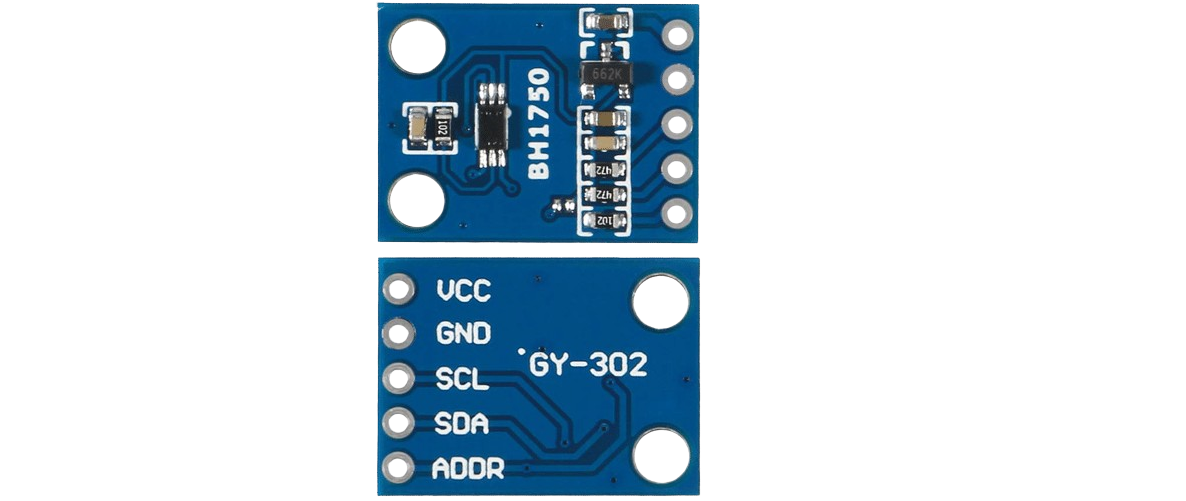
\includegraphics[width=16cm]{figuras/BH1750.png}
    \fonte{Retirado de \textcite{BH1750}.}
  \end{varwidth}
\end{figure}

\begin{table}[!htb]
    \caption{Especificações técnicas do sensor BH1750}
    \begin{tabularx}{\textwidth}{|X|X|} \hline
        \textbf{Parâmetro} & \textbf{Detalhes} \\ \hline
        Faixa de operação & 0-65535 lx \\ \hline
        Precisão & $\pm$0.24 lx  \\ \hline
        Resolução/Sensibilidade & Alta Resolução: 1 lx; Baixa Resolução: 4 lx \\ \hline
        Período de amostragem & Alta Resolução: 120-180 ms; Baixa Resolução: 16-24 ms \\ \hline
        Dimensões & 13.9x18.5 mm \\ \hline
    \end{tabularx}
    \label{tab:bh1750}
    \fonte{Retirado de \textcite{BH1750}.}
\end{table}

\subsection{Anemômetro RS-FSJT-N01}

O anemômetro RS-FSJT-N01 (Figura \ref{figura:anemometro}) é utilizado para medir a velocidade do vento. Ele opera por meio do protocolo Modbus RTU sobre RS485, enviando os dados de velocidade em m/s. Para a integração ao ESP32, foi necessário o uso do módulo conversor RS485 para TTL, que possibilita a comunicação compatível com os níveis lógicos do microcontrolador. Na Tabela \ref{tab:anemometro}, são apresentadas as especificações técnicas do anemômetro.

O anemômetro RS-FSJT-N01 foi selecionado devido à sua precisão na medição da velocidade do vento, um dos parâmetros utilizados em estudos meteorológicos e ambientais \parencite{Prathibha_system2017,Amine_system2024}. A velocidade do vento influencia diretamente fenômenos como a dispersão de poluentes, a sensação térmica e o transporte de umidade na atmosfera \parencite{Zhang_evapotranspiration_med2016}. Este modelo específico utiliza o protocolo Modbus RTU sobre RS485, uma tecnologia que garante comunicação confiável em ambientes sujeitos a ruído eletromagnético \parencite{ANEMOMETER}.

\begin{figure}[!htb] \centering
  \caption{Anemômetro RS-FSJT-N01} \label{figura:anemometro}
  \begin{varwidth}{\linewidth}
    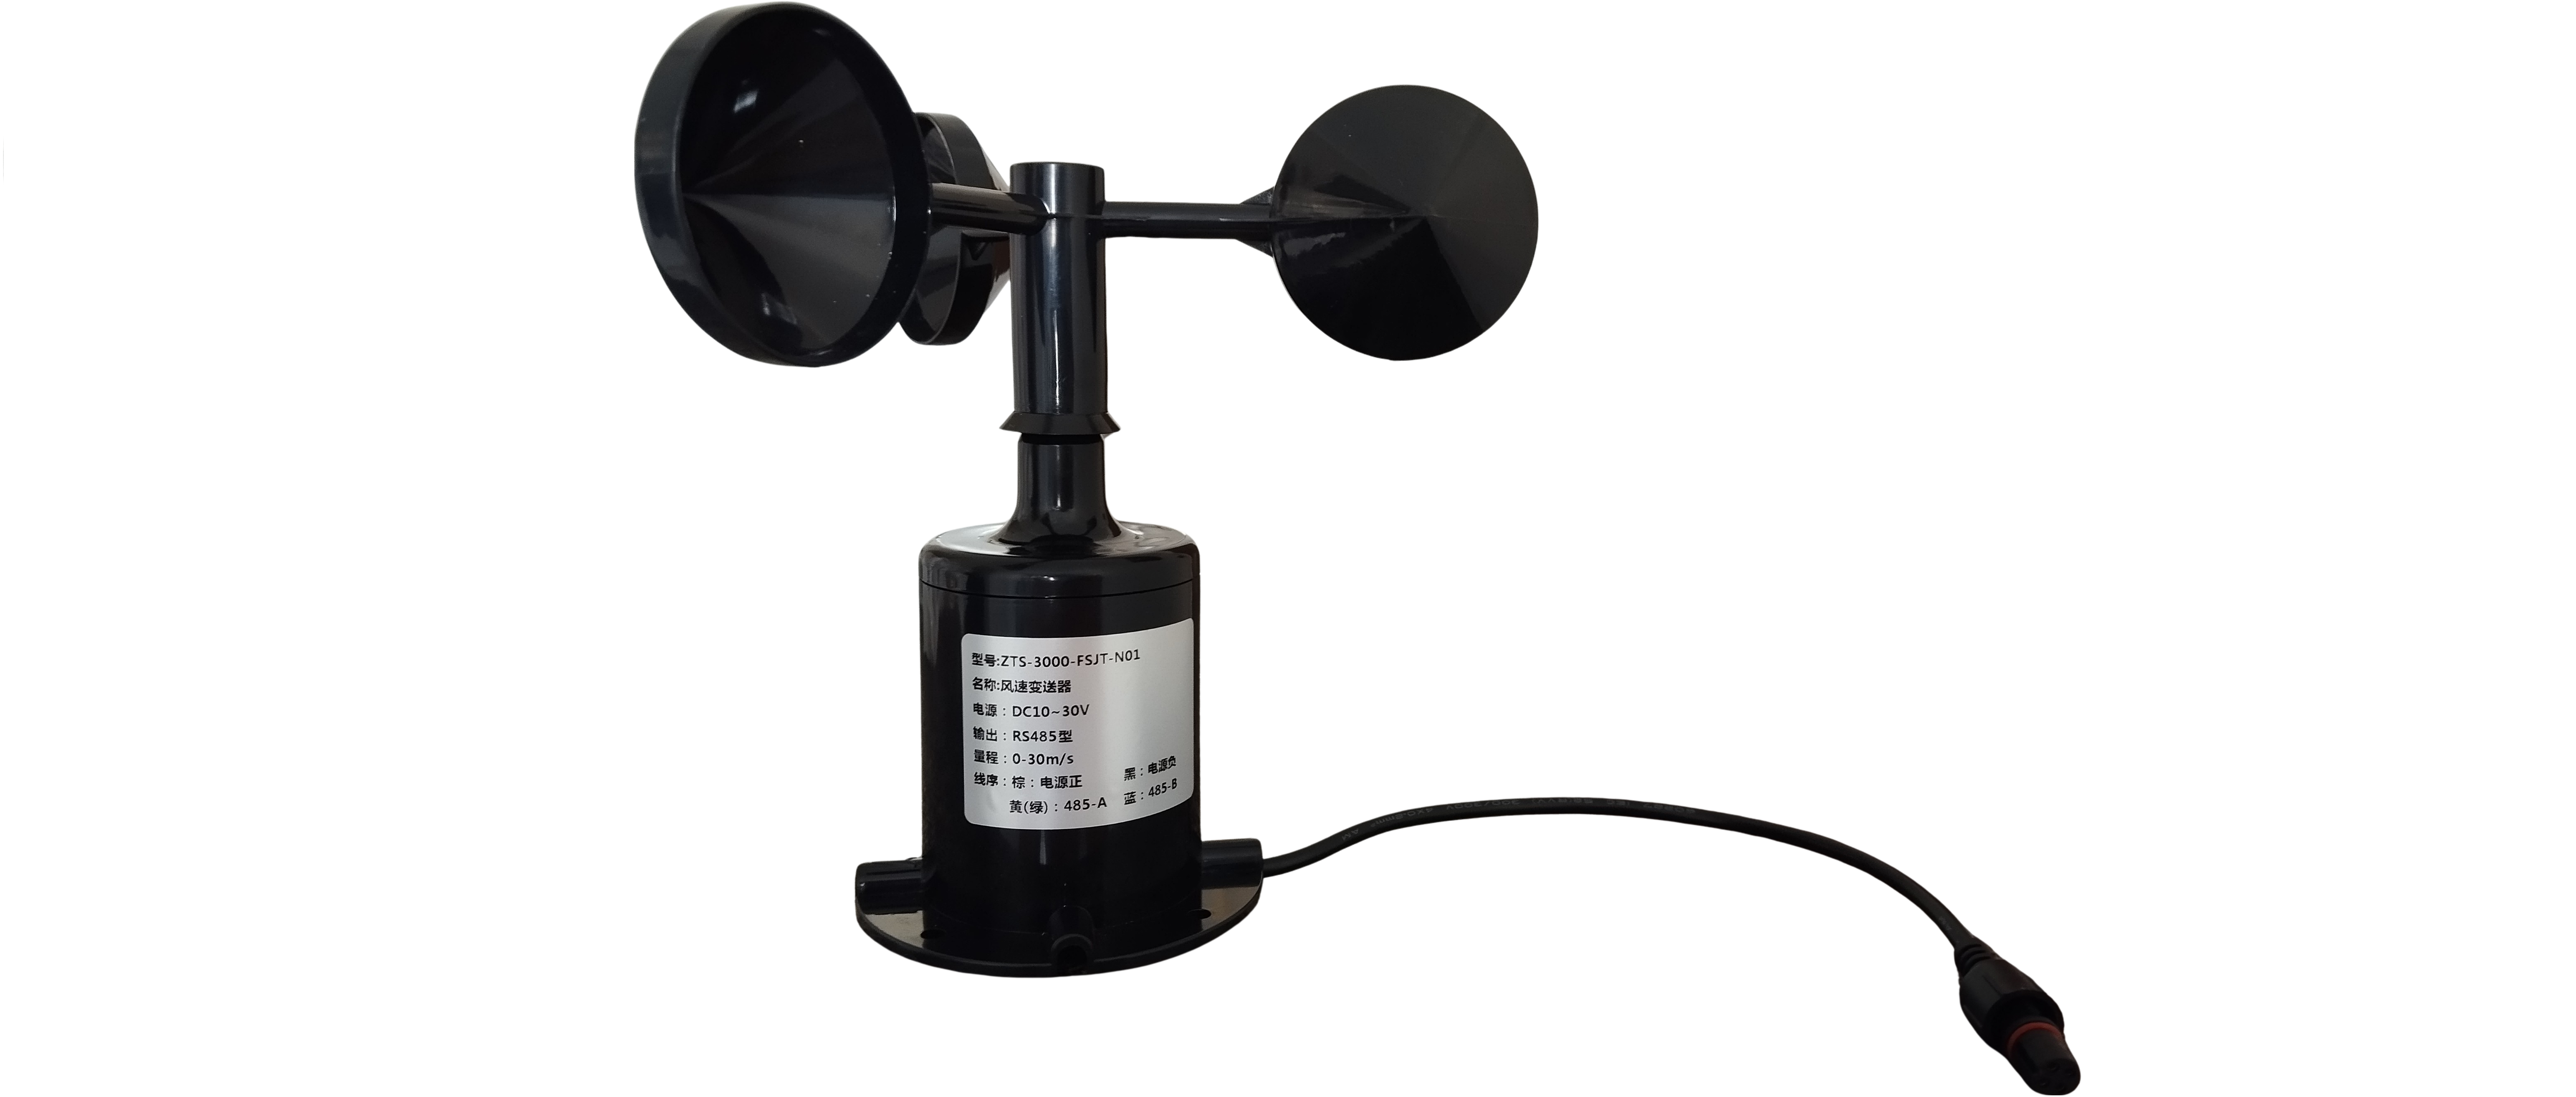
\includegraphics[width=16cm]{figuras/Anemometer.png}
    \fonte{Retirado de \textcite{ANEMOMETER}.}
  \end{varwidth}
\end{figure}

\begin{table}[!htb]
    \caption{Especificações técnicas do Anemômetro RS-FSJT-N01}
    \begin{tabularx}{\textwidth}{|X|X|} \hline
        \textbf{Parâmetro} & \textbf{Detalhes} \\ \hline
        Faixa de operação & 0-30 m/s \\ \hline
        Precisão & $\pm$0.3 m/s  \\ \hline
        Resolução/Sensibilidade & 0.1 m/s \\ \hline
        Período de amostragem & $\leq$ 1 s \\ \hline
        Dimensões & 182x80x160 mm \\ \hline
    \end{tabularx}
    \label{tab:anemometro}
    \fonte{Retirado de \textcite{ANEMOMETER}.}
\end{table}

\subsection{Comparador de Umidade do Solo LM393}

O módulo LM393 (Figura \ref{figura:lm393}) detecta a presença de umidade no solo com base na variação de condutividade elétrica. Ele foi conectado ao pino GPIO 13 do ESP32, configurado como entrada digital. Para alimentação, o módulo foi conectado ao pino 3V3 e ao GND do ESP32.

Para solos úmidos (acima de 50\% de umidade), o módulo fornece um sinal digital baixo (0), enquanto, para solos secos (abaixo de 50\% de umidade), o sinal é alto (1). O limiar de umidade pode ser ajustado através do potenciômetro presente no módulo usando-se uma chave \textit{philips}.

O comparador LM393 foi escolhido por ser ajustável e sensível a variações de umidade no solo \parencite{LM393}. A umidade do solo é um fator importante no contexto da irrigação, influenciando diretamente a absorção de nutrientes pelas plantas \parencite{Zhang_evapotranspiration_med2016}. O LM393 permite a detecção rápida e precisa de mudanças na umidade do solo, tornando a coleta em tempo real mais eficiente. Na Tabela \ref{tab:lm393}, são apresentadas as especificações técnicas do comparador.

\begin{figure}[!htb] \centering
  \caption{Comparador de umidade do solo LM393} \label{figura:lm393}
  \begin{varwidth}{\linewidth}
    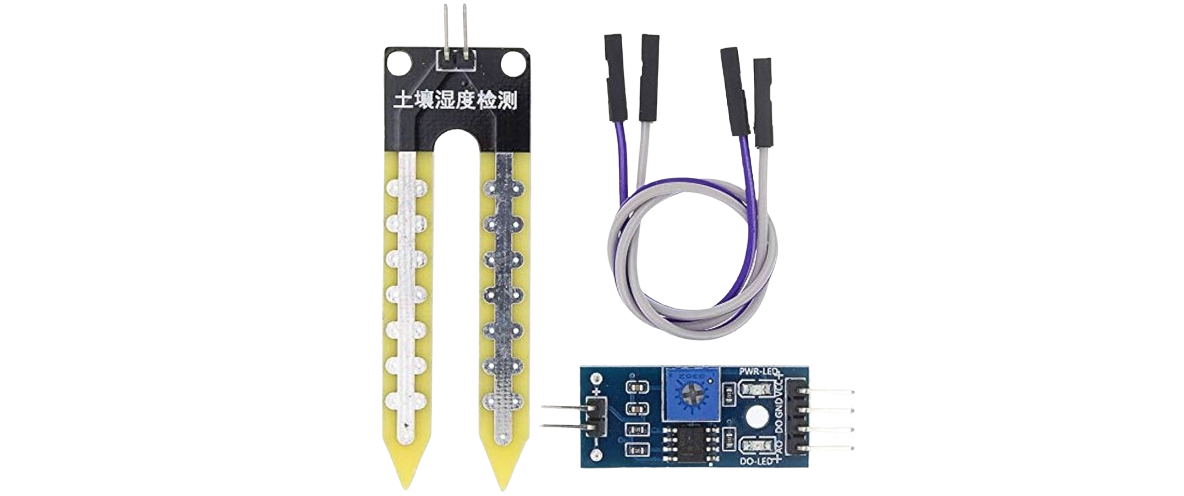
\includegraphics[width=16cm]{figuras/LM393.png}
    \fonte{Retirado de \textcite{LM393}.}
  \end{varwidth}
\end{figure}

\begin{table}[!htb]
  \caption{Especificações técnicas do Comparador LM393}
  \begin{tabularx}{\textwidth}{|X|X|} \hline
      \textbf{Parâmetro} & \textbf{Detalhes} \\ \hline
      Faixa de operação & 2.0 V a 36 V \\ \hline
      Precisão & $\pm$5.0 mV \\ \hline
      Resolução/Sensibilidade & 5 nA (corrente de offset) \\ \hline
      Período de amostragem & $\leq$ 1.3 $\mu$s \\ \hline
      Dimensões & 99x16 mm \\ \hline
  \end{tabularx}
  \label{tab:lm393}
  \fonte{Retirado de \textcite{LM393}.}
\end{table}

\subsection{Módulo GPS NEO-6M V2}

O módulo GPS NEO-6M (Figura \ref{figura:neo6m}) fornece informações de localização (latitude, longitude e altitude). Ele foi conectado ao ESP32 utilizando-se os pinos GPIO 18 e 19 para TX e RX, respectivamente. No código, os pinos foram configurados como \texttt{RX0} e \texttt{TX0}, empregando-se o protocolo UART para comunicação serial. Para alimentação, o módulo também foi conectado ao pino 3V3 e ao GND do ESP32.

O módulo GPS NEO-6M foi escolhido por sua capacidade de obtenção de coordenadas geográficas \parencite{NEO6M}. Essa funcionalidade permite a correlação de dados meteorológicos com a posição geográfica, facilitando a análise de padrões climáticos \parencite{Zhang_evapotranspiration_med2016}. O NEO-6M oferece uma precisão de até 2.5 metros, adequada para aplicações que requerem um rastreio preciso da localização \parencite{NEO6M}. Na Tabela \ref{tab:neo6}, são apresentadas as especificações técnicas do módulo.

\begin{figure}[!htb] \centering
  \caption{Módulo GPS NEO-6M V2} \label{figura:neo6m}
  \begin{varwidth}{\linewidth}
    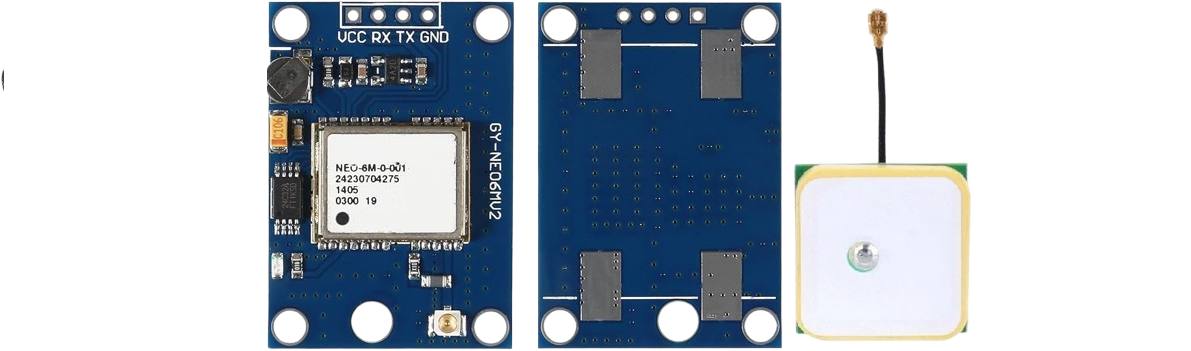
\includegraphics[width=16cm]{figuras/NEO6MV2.png}
    \fonte{Retirado de \textcite{NEO6M}.}
  \end{varwidth}
\end{figure}

\begin{table}[!htb]
  \caption{Especificações técnicas do Módulo GPS NEO-6M V2}
  \begin{tabularx}{\textwidth}{|X|X|} \hline
      \textbf{Parâmetro} & \textbf{Detalhes} \\ \hline
      Faixa de operação & 2.7 V a 3.6 V \\ \hline
      Precisão & 2.5 m (GPS), 2.0 m (SBAS) \\ \hline
      Resolução/Sensibilidade & -161 dBm \\ \hline
      Período de amostragem & Até 5 Hz \\ \hline
      Dimensões & 16x12.2x2.4 mm \\ \hline
  \end{tabularx}
  \label{tab:neo6}
  \fonte{Retirado de \textcite{NEO6M}.}
\end{table}

\subsection{Módulo Conversor RS485 para TTL}

O módulo conversor RS485 para TTL (Figura \ref{figura:ttl_rs485}) é utilizado para conectar o ESP32 ao anemômetro RS-FSJT-N01, convertendo os sinais TTL para níveis compatíveis com RS485 \parencite{RS485TTL}. Ele foi conectado ao ESP32 usando-se os pinos GPIO 16 e 17 (TX e RX), que eram ligados aos pinos RXD e TXD do módulo, respectivamente. Já o barramento RS485 do anemômetro conectado aos terminais A e B do módulo e a alimentação deste foram feitos por uma fonte de 12V genérica. No código, os pinos foram configurados como \texttt{MAX485\_RX} e \texttt{MAX485\_TX}, para a comunicação serial. Na Tabela \ref{tab:rs485}, são apresentadas as especificações técnicas do módulo.

\begin{figure}[!htb] \centering
  \caption{Módulo Conversor RS485 para TTL} \label{figura:ttl_rs485}
  \begin{varwidth}{\linewidth}
    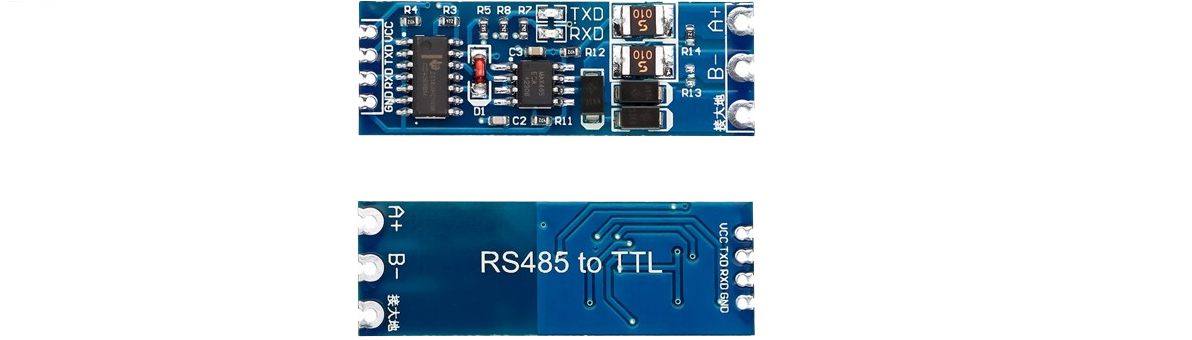
\includegraphics[width=16cm]{figuras/TTL_TO_RS485.png}
    \fonte{Retirado de \textcite{RS485TTL}.}
  \end{varwidth}
\end{figure}

\begin{table}[!htb]
  \caption{Especificações técnicas do Módulo Conversor RS485 para TTL}
  \begin{tabularx}{\textwidth}{|X|X|} \hline
      \textbf{Parâmetro} & \textbf{Detalhes} \\ \hline
      Faixa de operação & 5 V \\ \hline
      Dimensões & 44x14 mm \\ \hline
  \end{tabularx}
  \label{tab:rs485}
  \fonte{Retirado de \textcite{RS485TTL}.}
\end{table}

\subsection{Custos dos Componentes}

Os custos dos componentes utilizados no desenvolvimento desse sistema podem variar de acordo com o fornecedor, região de compra e período de aquisição. A Tabela \ref{tab:custos} apresenta os custos dos componentes utilizados, já com os impostos e taxas de importação inclusos. Os componentes foram comprados por meio da loja virtual \textit{AliExpress} no dia 17/06/2024.

\begin{table}[!htb]
  \caption{Custos dos componentes utilizados no sistema}
  \begin{tabularx}{\textwidth}{|X|X|} \hline
      \textbf{Componente} & \textbf{Custo (R\$)} \\ \hline
      ESP32 & 20,19 \\ \hline
      DHT22 & 7,66 \\ \hline
      BMP280 & 4,65 \\ \hline
      BH1750 & 6,04 \\ \hline
      Anemômetro RS-FSJT-N01 & 100,43 \\ \hline
      LM393 & 4,64 \\ \hline
      NEO-6M & 22,89 \\ \hline
      Conversor RS485 para TTL & 10,86 \\ \hline
      \textbf{Total} & \textbf{177,36} \\ \hline
  \end{tabularx}
  \label{tab:custos}
  \fonte{Elaborado pelo autor, 2024.}
\end{table}


\section{Integração dos sensores ao ESP32}

Como foram utilizados sensores para capturar os dados, é importante destacar que todo instrumento de medição possui erros inerentes \parencite{Vuolo_erro1996}, que podem ser classificados em dois tipos:

\begin{itemize} 
    \item Erros sistemáticos, sendo estes previsíveis e reproduzíveis. Normalmente, são originados de falhas no próprio instrumento de medição ou de influências ambientais que afetam de maneira constante o resultado. Eles podem ser corrigidos através de calibração e ajustes do sistema;
    \item Erros estatísticos, que, diferentemente dos erros sistemáticos, ocorrem de forma aleatória e imprevisível. São, geralmente, causados por flutuações nas condições de medição, como ruído no sinal ou variações no ambiente. Eles não podem ser eliminados por calibração, mas podem ser reduzidos por meio da repetição e tratamento estatístico dos dados. 
\end{itemize}

Neste trabalho, cada sensor passou um teste individual de leitura por um período de 24 horas. Tanto antes quanto depois dos testes, os sensores mantiveram sua operação normal e dentro do esperado de suas especificações técnicas. Isso foi feito a fim de observar e minimizar possíveis erros sistemáticos e garantir o funcionamento ininterrupto dos sensores.

Por fim, os componentes foram integrados em um sistema cyberfísico que publica as leituras individuais de cada sensor em um \textit{broker}. Neste trabalho, optou-se pelo EMQX (Figura \ref{figura:emqx}), uma plataforma de código aberto para MQTT \parencite{EMQX}.

\begin{figure}[!htb] \centering
  \caption{Interface da plataforma EMQX} \label{figura:emqx}
  \begin{varwidth}{\linewidth}
    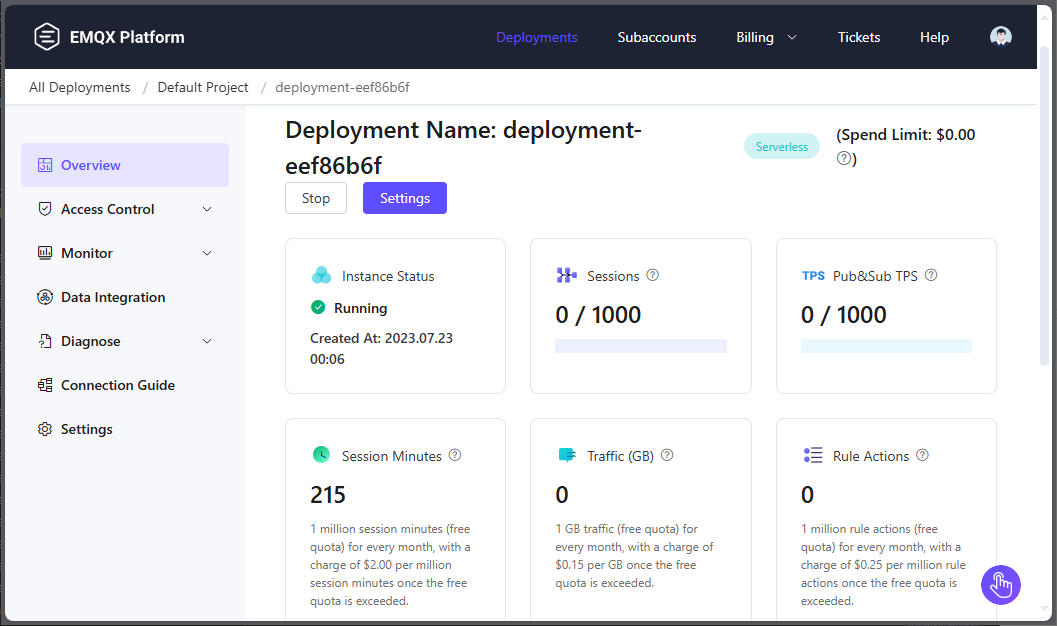
\includegraphics[width=16cm]{figuras/emqx.png}
    \fonte{Elaborado pelo autor, 2024.}
  \end{varwidth}
\end{figure}

Nele, as mensagens são distribuídas em tópicos usando-se protocolos de comunicação (MQTT) e criptografia (TLS). Isso garante a integridade e a confidencialidade dos dados coletados, além do acesso remoto e em tempo real às leituras. Este acesso é feito através da conexão entre o \textit{broker} e o \textit{backend} do sistema, que se inscreve nos tópicos de interesse para receber os dados. Também é feita uma segunda instância de armazenamento em um banco de dados relacional (\textit{MySQL}) para consultas de interesse. 

O armazenamento dos dados históricos no \textit{MySQL} é realizado por meio da funcionalidade de \textit{Rule Engine} do EMQX, que permite criar regras para processar as mensagens recebidas. Por meio dessas regras, as mensagens publicadas nos tópicos são capturadas e inseridas em uma tabela no banco (\texttt{mqtt\_messages}), previamente configurada com colunas \textit{topic}, \textit{payload}, \textit{qos} e \textit{timestamp}. Esse mecanismo permite a persistência dos dados e possibilita consultas históricas para análises ou monitoramento posterior.

\section{Ferramentas e Tecnologias Utilizadas}

Para o desenvolvimento do sistema proposto neste trabalho, foram empregadas ferramentas e tecnologias, cada uma com seus papéis específicos.

\subsection{Linguagem \textit{C}}
A linguagem de programação \textit{C} foi utilizada para o desenvolvimento do \textit{firmware} do ESP32. Essa escolha deve-se à sua proximidade com o \textit{hardware}, permitindo maior controle sobre os recursos embarcados. Além disso, o \textit{C} é suportado nativamente por diversas plataformas de desenvolvimento, o que facilita a portabilidade do código.

No desenvolvimento do \textit{firmware}, diversas bibliotecas foram empregadas para simplificar a implementação e assegurar a confiabilidade das funcionalidades. Abaixo, são listadas as principais bibliotecas utilizadas:

\begin{itemize}
    \item \texttt{Arduino}: biblioteca base para desenvolvimento com a plataforma Arduino, fornecendo funções para manipulação de pinos, comunicação serial e temporização.
    \item \texttt{ModbusMaster}: implementação do protocolo Modbus RTU, permitindo comunicação entre dispositivos escravos e mestres em redes industriais.
    \item \texttt{Wire}: biblioteca utilizada para comunicação I2C, facilitando a integração com sensores e dispositivos externos.
    \item \texttt{WiFi}: biblioteca nativa para gerenciar conexões Wi-Fi no ESP32, necessária para conectividade com redes locais e a \textit{internet}.
    \item \texttt{Adafruit\_Sensor} e \texttt{Adafruit\_BMP280}: fornecem suporte para leitura de dados ambientais de sensores como o BMP280, usado para medir pressão atmosférica e temperatura.
    \item \texttt{DHT} e \texttt{DHT\_U}: bibliotecas dedicadas a sensores de temperatura e umidade da linha DHT (por exemplo, DHT11 ou DHT22).
    \item \texttt{BH1750}: biblioteca para integração com o sensor de luz BH1750, utilizado para medições de luminosidade.
    \item \texttt{WiFiClientSecure}: extensão da biblioteca Wi-Fi para conexões utilizando TLS/SSL, garantindo comunicações criptografadas.
    \item \texttt{PubSubClient}: implementação do protocolo MQTT, necessário para a comunicação com o \textit{backend}.
    \item \texttt{TinyGPSPlus}: biblioteca para interpretação de dados recebidos de módulos GPS, necessários para obter informações de localização geográfica.
\end{itemize}

A combinação dessas bibliotecas permitiu a criação de um \textit{firmware} capaz de monitorar e controlar diversos sensores e atuadores, além de garantir conectividade e comunicação com sistemas externos.

\subsection{\textit{Node.js}}
O ambiente de execução \textit{Node.js} foi empregado no desenvolvimento do \textit{backend} devido à sua capacidade de gerenciar múltiplas conexões simultâneas. \textit{Node.js} é particularmente adequado para aplicações que exigem baixa latência, como em sistemas em tempo real.

No desenvolvimento do \textit{backend}, foram usadas diversas bibliotecas para otimizar funcionalidades e assegurar boas práticas de programação. A seguir, são destacadas as principais dependências e suas funções no projeto:

\begin{itemize}
    \item \texttt{Express}: \textit{Framework} para construção de servidores \textit{web}, usado para gerenciar rotas e requisições HTTP.
    \item \texttt{Axios}: Biblioteca empregada para realizar requisições HTTP, facilitando a comunicação com APIs externas.
    \item \texttt{Cors}: \textit{Middleware} que permite configurar políticas de compartilhamento de recursos entre diferentes origens, necessário para integrar o \textit{frontend} com o \textit{backend}.
    \item \texttt{Dotenv}: biblioteca usada para gerenciar variáveis de ambiente, permitindo a configuração de credenciais e configurações do sistema.
    \item \texttt{MQTT}: protocolo para comunicação em tempo real, empregado no gerenciamento de mensagens entre dispositivos conectados.
    \item \texttt{Zod}: biblioteca para validação e definição de esquemas de dados, assegurando a integridade das entradas e saídas da aplicação.
\end{itemize}

Além das dependências de produção, foi utilizada uma estrutura de dependências de desenvolvimento para garantir qualidade no código e simplificar o processo:

\begin{itemize}
    \item \texttt{Typescript}: \textit{Superset} do JavaScript que adiciona tipagem estática ao código, prevenindo erros.
    \item \texttt{Jest} e \texttt{Supertest}: ferramentas para testes automatizados que permitem validar funcionalidades e garantir o funcionamento correto da aplicação.
    \item \texttt{ESLint} e \texttt{Prettier}: configurações para impor boas práticas de codificação e formatação consistente, otimizando a legibilidade e manutenção do código.
    \item \texttt{Nodemon} e \texttt{ts-node}: facilitam o desenvolvimento ao permitir recarga automática do servidor e execução de arquivos TypeScript sem necessidade de transpilação prévia.
\end{itemize}

Esse conjunto de ferramentas proporcionou um ambiente de desenvolvimento produtivo e um \textit{backend} eficiente, escalável e seguro.

\subsection{\textit{Next.js}}
A biblioteca \textit{Next.js} foi utilizada para o desenvolvimento da interface do \textit{frontend}, oferecendo uma arquitetura de renderização híbrida que combina renderização do lado do servidor - SSR (sigla do inglês, \textit{server-side rendering}) e renderização do lado do cliente - CSR (sigla do inglês, \textit{client-side rendering}). Isso permite que as páginas \textit{web} sejam renderizadas no servidor e enviadas para o cliente, proporcionando uma experiência de usuário rápida e responsiva. A seguir, destacam-se as principais dependências empregadas no projeto e suas funcionalidades:

\begin{itemize} 
  \item \texttt{@next/font}: utilizado para integrar fontes personalizadas diretamente no projeto, otimizando o desempenho no carregamento de fontes. 
  \item \texttt{@radix-ui/react-dropdown-menu}, \texttt{@radix-ui/react-scroll-area} e \texttt{@radix-ui/react-slot}: componentes acessíveis e estilizados para construção de interfaces reativas e intuitivas.
  \item \texttt{@tailwindcss/typography}: \textit{Plugin} do \textit{TailwindCSS} que adiciona estilos predefinidos para tipografia, simplificando a criação de layouts bem formatados. 
  \item \texttt{axios}: biblioteca utilizada para realizar requisições HTTP, integrando a interface com as APIs do \textit{backend}. 
  \item \texttt{class-variance-authority}: facilita a manipulação de classes CSS com base em variantes condicionais, permitindo maior flexibilidade no estilo. 
  \item \texttt{clsx}: utilizado para combinar classes CSS dinamicamente, de maneira concisa e legível. 
  \item \texttt{lucide-react}: biblioteca de ícones leves e modernos, utilizada para enriquecer a interface visual. 
  \item \texttt{next-themes}: fornece suporte à alternância entre temas claros e escuros, aprimorando a experiência do usuário. 
  \item \texttt{react-icons}: conjunto abrangente de ícones para \textit{React}, permitindo a inclusão de gráficos contextuais no \textit{design}. 
  \item \texttt{react-responsive-carousel}: componente de carrossel responsivo para exibição de imagens ou conteúdos de forma dinâmica. 
  \item \texttt{sharp}: biblioteca para manipulação de imagens no lado do servidor, otimizando tamanhos e formatos para diferentes dispositivos. 
  \item \texttt{tailwind-merge}: facilita a mesclagem de classes \textit{TailwindCSS}, ajudando a resolver conflitos de estilo. 
  \item \texttt{tailwindcss-animate}: \textit{Plugin} que adiciona animações ao \textit{TailwindCSS}, tornando a experiência do usuário mais fluida e atraente. 
  \item \texttt{zod}: biblioteca para validação e definição de esquemas de dados, assegurando a integridade das informações manipuladas no \textit{frontend}. \end{itemize}

Para garantir qualidade e consistência durante o desenvolvimento, foram empregadas diversas dependências de ambiente:

\begin{itemize} 
  \item \texttt{@types/node}, \texttt{@types/react} e \texttt{@types/react-dom}: adicionam tipagem para as bibliotecas principais, garantindo integração com o \texttt{Typescript}. 
  \item \texttt{autoprefixer}: automatiza a inclusão de prefixos de compatibilidade para navegadores, assegurando suporte abrangente ao CSS. 
  \item \texttt{eslint} e \texttt{eslint-config-next}: ferramentas de análise de código estático que impõem boas práticas no desenvolvimento. 
  \item \texttt{eslint-config-prettier}: garante integração entre o \texttt{ESLint} e o \texttt{Prettier}, evitando conflitos entre as regras. 
  \item \texttt{postcss}: Processador CSS que melhora a compatibilidade e otimização dos estilos. 
  \item \texttt{prettier}: ferramenta de formatação automática, assegurando consistência visual no código. 
  \item \texttt{tailwindcss}: \textit{Framework} de utilitários CSS que acelera o desenvolvimento de estilos responsivos e customizados. 
  \item \texttt{typescript}: adiciona tipagem estática ao JavaScript, prevenindo erros comuns e proporcionando maior robustez ao código. \end{itemize}

Esse conjunto de ferramentas e dependências permitiu o desenvolvimento de um \textit{frontend} moderno, dinâmico e escalável, com foco na experiência do usuário e na eficiência do sistema.

\subsection{\textit{Jest}}
O \textit{framework} de testes \textit{Jest} foi adotado para a realização de testes automatizados. Essa ferramenta foi escolhida por sua simplicidade de configuração e pela capacidade de executar testes unitários e de integração, garantindo a qualidade e a confiabilidade do código, além de facilitar a manutenção e evolução do sistema.

A estrutura dos testes foi organizada em dois principais níveis, separados por pastas, para maior clareza e modularidade:

\begin{itemize}
  \item Ponta a ponta: contém testes que verificam o funcionamento completo da aplicação em cenários reais, cobrindo desde as requisições feitas ao servidor até as respostas entregues. No sistema implementado nesta pesquisa, o teste avalia o comportamento do sistema como um todo, validando o fluxo de dados entre os componentes.
  \item Unitários: reúne testes focados em unidades específicas do sistema, como funções, serviços ou classes individuais. Cada teste nesta pasta avalia o comportamento isolado de componentes-chave, garantindo que funcionem conforme o esperado. Nesta pesquisa, os testes unitários foram utilizados para validar a lógica de negócio e o transporte dos dados entre as camadas do sistema.
\end{itemize}

Essa organização entre testes de integração e testes unitários permite isolar falhas e assegurar que tanto os componentes individuais quanto a aplicação como um todo funcionem de forma consistente e modular.

\subsection{\textit{Shadcn/ui}}
A biblioteca de componentes \textit{Shadcn/ui} foi utilizada no desenvolvimento do \textit{frontend}, proporcionando componentes reutilizáveis e estilizados que aceleraram o processo de construção da interface. Essa biblioteca foi selecionada por sua flexibilidade e integração nativa com o \textit{framework} \textit{TailwindCSS}. Neste trabalho, foram usados os seguintes componentes:
\begin{itemize}
  \item \texttt{Button}: botão interativo com estilos personalizáveis e animações integradas.
  \item \texttt{Badge}: indicador visual para destacar informações importantes.
  \item \texttt{Card}: cartão de conteúdo com layout flexível e responsivo.
  \item \texttt{Dropdown-menu}: menu suspenso com opções personalizáveis e animações suaves.
  \item \texttt{Scroll-area}: área de rolagem personalizada com suporte a conteúdo dinâmico.
  \item \texttt{Skeleton}: efeito de carregamento para indicar que o conteúdo está sendo carregado.
\end{itemize}

\subsection{\textit{TailwindCSS}}
O \textit{framework} \textit{TailwindCSS} foi empregado na estilização do \textit{frontend}. Sua abordagem utilitária permite a criação de interfaces consistentes e bem estilizadas de maneira rápida e eficiente, o que foi importante para garantir um \textit{design} responsivo e atrativo. Neste travalho, foram utilizadas paletas de cores voltadas para o uso em ambientes externos, com tons de verde e branco destacados.

\subsection{Figma}
A ferramenta Figma (Figura \ref{figura:figma}) foi empregada na prototipagem de interfaces gráficas. Sua escolha foi motivada pela variedade de recursos disponíveis para o \textit{design} e validação de interfaces antes de sua implementação.

\begin{figure}[!htb] \centering
  \caption{Interface da aplicação Figma} \label{figura:figma}
  \begin{varwidth}{\linewidth}
    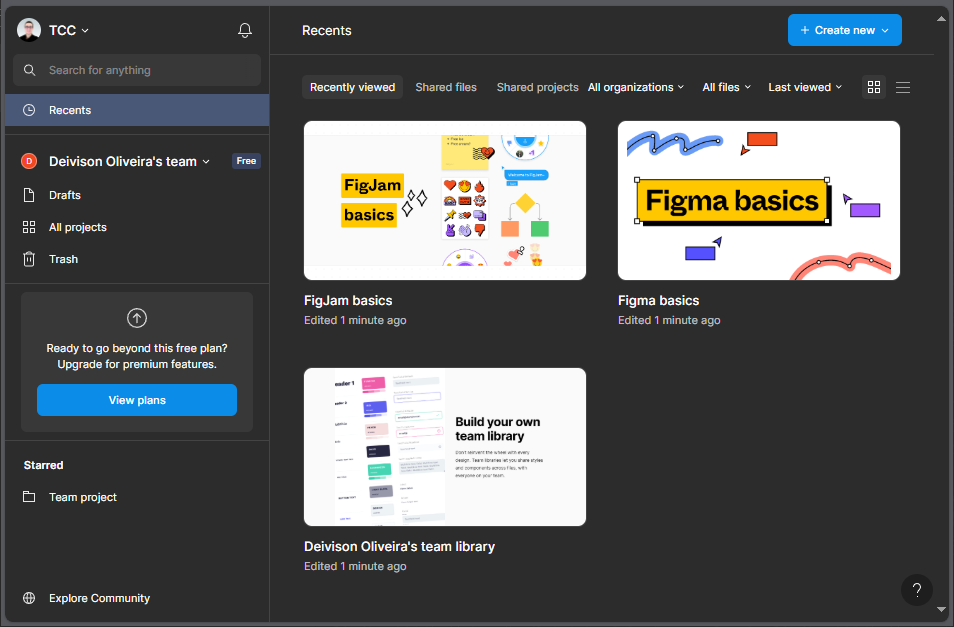
\includegraphics[width=16cm]{figuras/figma.png}
    \fonte{Elaborado pelo autor, 2024.}
  \end{varwidth}
\end{figure}

\subsection{Visual Studio Code}
O Visual Studio Code (Figura \ref{figura:vscode}) foi empregado como ambiente de desenvolvimento integrado - IDE (sigla do inglês \textit{Integrated Development Environment}) para o desenvolvimento do \textit{frontend} e do \textit{backend}. Essa ferramenta foi escolhida por sua versatilidade, extensibilidade e suporte a diversas linguagens e tecnologias, incluindo as mencionadas neste trabalho.

\begin{figure}[!htb] \centering
  \caption{Interface do Visual Studio Code} \label{figura:vscode}
  \begin{varwidth}{\linewidth}
    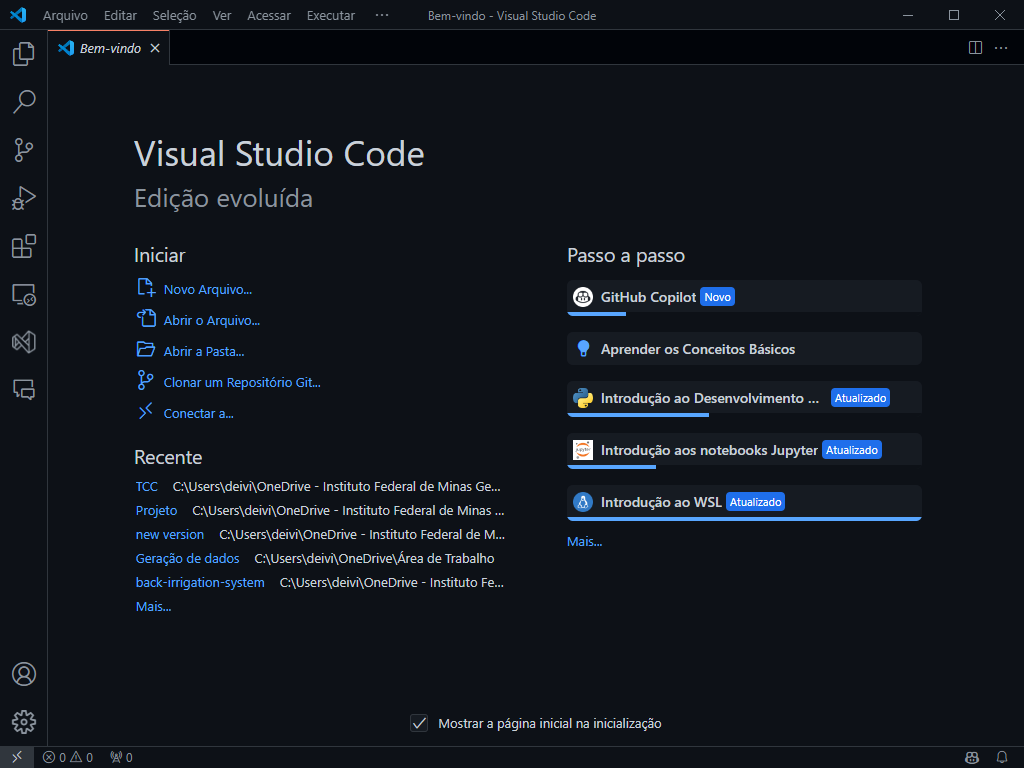
\includegraphics[height=10cm, width=16cm]{figuras/vscode.png}
    \fonte{Elaborado pelo autor, 2024.}
  \end{varwidth}
\end{figure}

\subsection{Arduino IDE}
A Arduino IDE (Figura \ref{figura:arduino-ide}) foi utilizada como IDE para o desenvolvimento embarcado no ESP32. Essa escolha se justifica pela usabilidade da ferramenta e pela compatibilidade com a plataforma ESP32, facilitando a criação e a depuração do \textit{firmware}.

\begin{figure}[!htb] \centering
  \caption{Interface do Arduino IDE} \label{figura:arduino-ide}
  \begin{varwidth}{\linewidth}
    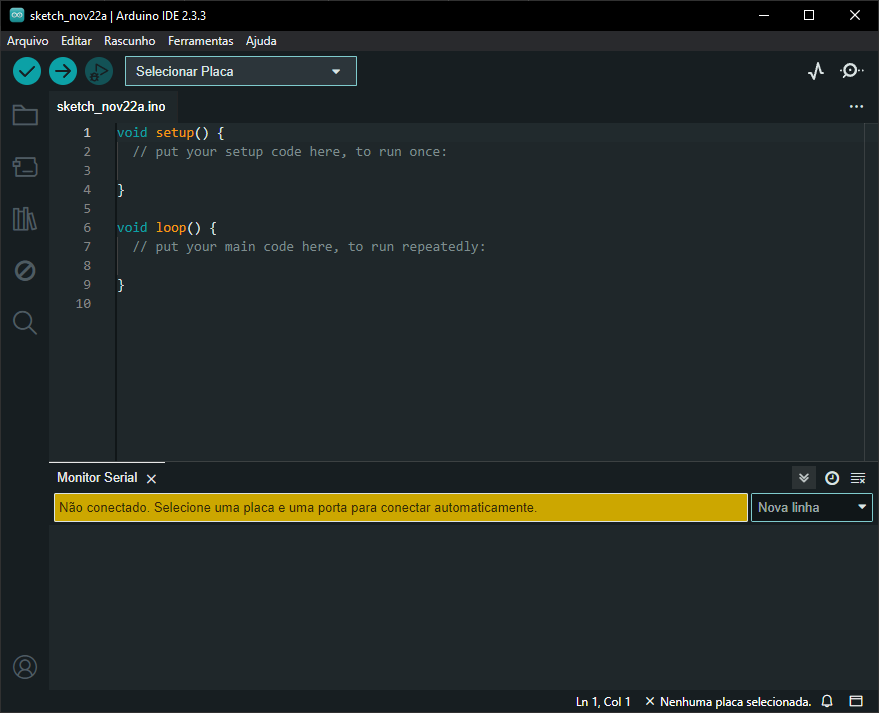
\includegraphics[height=10cm, width=16cm]{figuras/arduino-ide.png}
    \fonte{Elaborado pelo autor, 2024.}
  \end{varwidth}
\end{figure}

\subsection{Fritzing}
O Fritzing (Figura \ref{figura:fritzing}) foi empregado na prototipagem de circuitos eletrônicos. Essa ferramenta permite a criação de esquemas e \textit{layouts} de circuitos de maneira intuitiva, sendo necessária para a validação do \textit{hardware} antes de sua implementação definitiva.

\begin{figure}[!htb] \centering
  \caption{Interface da aplicação Fritzing} \label{figura:fritzing}
  \begin{varwidth}{\linewidth}
    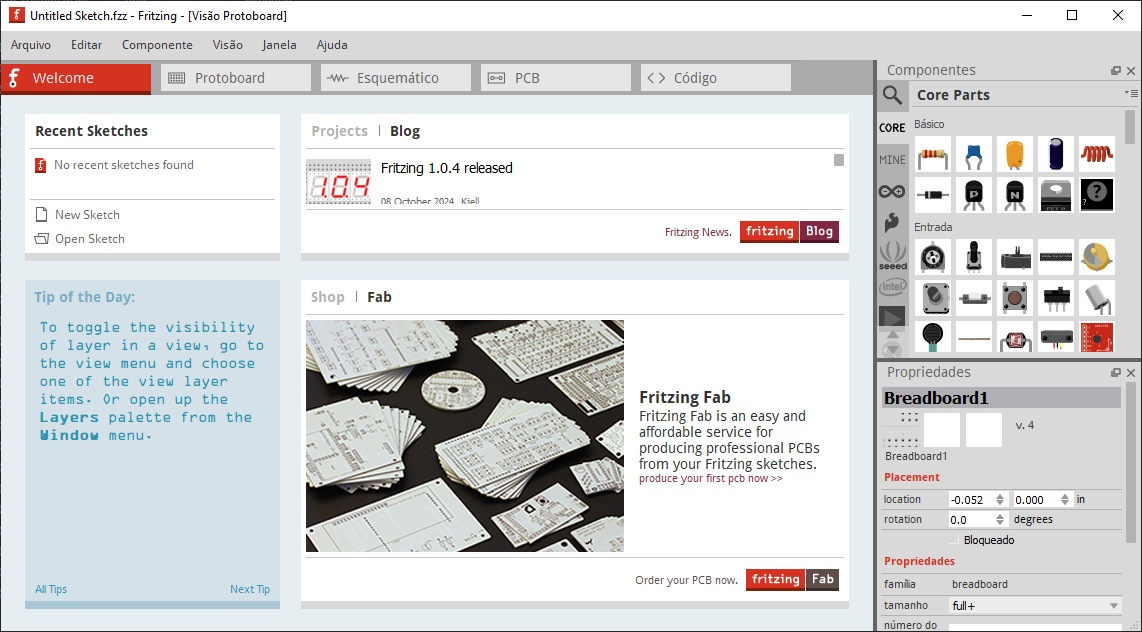
\includegraphics[width=16cm]{figuras/fritzing.png}
    \fonte{Elaborado pelo autor, 2024.}
  \end{varwidth}
\end{figure}

\subsection{EasyEDA}
A ferramenta EasyEDA (Figura \ref{figura:easyeda}) foi utilizada para o desenho das placas de circuito impresso - PCB (sigla do inglês \textit{Printed Circuit Board}). Sua escolha foi motivada pela facilidade de uso e pelos recursos para simulação e validação de projetos eletrônicos, garantindo a qualidade e a confiabilidade das placas desenvolvidas.

\begin{figure}[!htb] \centering
  \caption{Interface da aplicação EasyEDA} \label{figura:easyeda}
  \begin{varwidth}{\linewidth}
    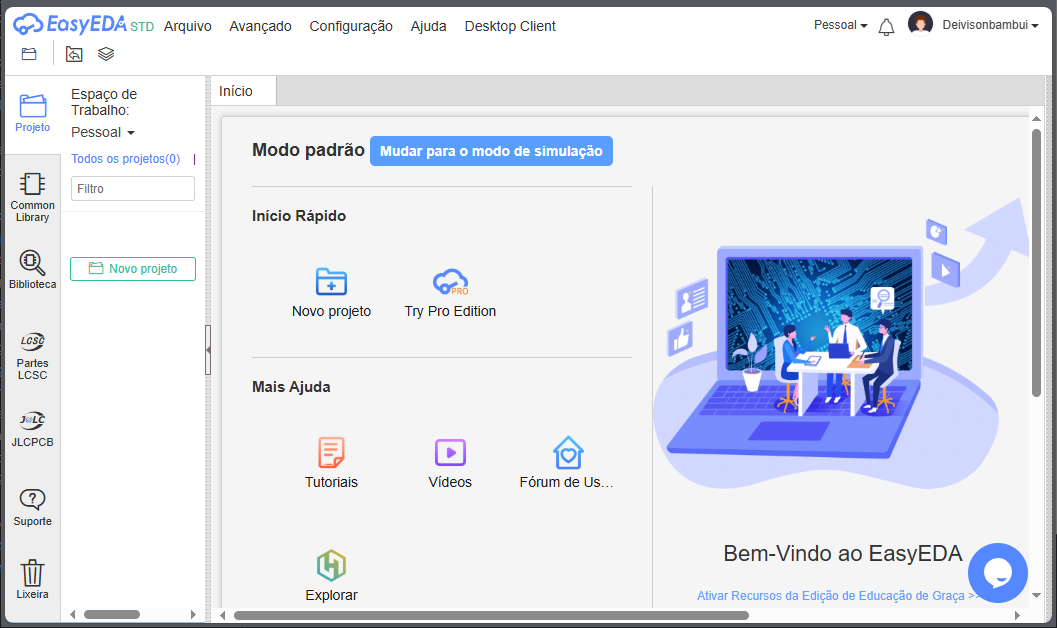
\includegraphics[width=16cm]{figuras/easyeda.png}
    \fonte{Elaborado pelo autor, 2024.}
  \end{varwidth}
\end{figure}

\subsection{Resumo das escolhas}
As tecnologias e ferramentas mencionadas foram selecionadas para atender aos requisitos específicos do sistema proposto, priorizando desempenho, escalabilidade e experiência prévia de desenvolvimento.

A análise dos dados meteorológicos é realizada de forma contínua para apresentar medições e cálculos estimativos de ETo e ETc locais. Esse método de análise permite a interpretação e avaliação dos dados de forma rápida, além de gerar relatórios periódicos para a tomada de decisões.

\section{Estimativa da evapotranspiração}

O cálculo da ETo e da ETc é usado para o monitoramento hídrico em tempo real e é realizado com base nas leituras dos sensores. Foram usadas as equações da FAO-56 apresentadas por \textcite{Allen_evapotranspiration1998} como modelagem referencial. Cada leitura dos sensores contribui diretamente para o cálculo dessas variáveis, ou é convertida de forma a ser utilizada na equação.

\subsection{Variáveis meteorológicas e sua obtenção}

As variáveis meteorológicas utilizadas no cálculo da evapotranspiração são obtidas da seguinte forma:
\begin{itemize}
    \item A temperatura do ar (\(T\)) é medida diretamente do sensor DHT22, que fornece a temperatura em graus Celsius;
    
    \item A umidade relativa (\(RH\)) também é medida pelo sensor DHT22, em percentual;
    
    \item A umidade do solo (\(h\)) é medida pelo comparador LM393 com eletrodos externos, em um intervalo analógico;
    
    \item A pressão atmosférica (\(P\)) é obtida do sensor BMP280, em hPa;

    \item A velocidade do vento (\(u_2\)) é medida pelo anemômetro, em m/s.
\end{itemize}

As demais variáveis são estimadas a partir de cálculos intermediários, obtidos, em sua maioria, da obra de \textcite{Allen_evapotranspiration1998}:
\begin{itemize}
    \item A radiação líquida (\(R_n\)) é estimada a partir das leituras do sensor de luminosidade BH1750, que mede a intensidade luminosa em lux a cada segundo. 
    \begin{itemize}
        \item \textcite{Michael_2020} apresentam a conversão de lux (\(lx\)) para irradiância solar (\(E\)) em W/m², dada pela equação:
        \[ E \approx \frac{lx}{120} \]

        \item A irradiância solar, por sua vez, é a própria radiação solar (\(R_s\)):
        
        \[ R_s = E \]

        \item Desta forma, é possível determinar a radiação líquida solar (\(R_{ns}\)), dada por:
        
        \[ R_{ns} = 0.77 \cdot R_s \]

        \item O último componente necessário para determinar a \(R_n\) é a radiação líquida de ondas longas (\(R_{nl}\)), que é resultante das seguintes equações:
        
        \begin{itemize}
            \item A distância relativa inversa Terra-Sol (\(d_r\)), que é calculada como:
            
            \[
            d_r = 1 + 0.033 \cos\left( \frac{2 \pi J}{365} \right)
            \]
            onde \(J\) é o dia do ano.
            
            \item A radiação extraterrestre por períodos horários ou mais curtos (\(R_a\)), dada por:
            
            \[
            R_a = \frac{12 \cdot 60}{\pi} G_{sc} d_r 
            \left[ 
            (\omega_2 - \omega_1) \sin(\phi) \sin(\delta) + 
            \cos(\phi) \cos(\delta) (\sin(\omega_2) - \sin(\omega_1)) 
            \right]
            \]
            onde \(G_{sc} = 0.0820 \, MJ \, m^{-2} \, min^{-1}\), \( \delta = 0.409 \sin\left( \frac{2 \pi J}{365} - 1.39 \right)\), \(\phi\) é o grau de latitute (obtido pelo módulo GPS NEO-6M V2), e os ângulos \( \omega_1 \) e \( \omega_2 \) são os ângulos de tempo solar no início e no final do período, respectivamente.
            
            \item A radiação solar com céu limpo (\(R_{so}\)), dada por:
            
            \[
            R_{so} = (0.75 + 2 \cdot 10^{-5} z) R_a
            \]
            onde \(z\) é a elevação, em metros, do nível do mar.
            
            \item A radiação líquida de ondas longas (\(R_{nl}\)), estimada por:
            
            \[
            R_{nl} = \sigma \left( \frac{T_{max,K}^4 + T_{min,K}^4}{2} \right) \left[ 0.34 - 0.14 \sqrt{e_a} \right] \left( 1.35 \frac{R_s}{R_{so}} - 0.35 \right)
            \]
            onde \(T_{max,K}\) e \(T_{min,K}\) são as temperaturas máxima e mínima em Kelvin, \( \sigma \) é a constante de Stefan-Boltzmann (\(4.903 \cdot 10^{-9} \, MJ \, K^{-4} \, m^{-2} \, dia^{-1} \)), e \(e_a\) é a pressão de vapor atual.
        \end{itemize}

        \item A \(R_n\) resultante é dada por:
        
        \[ R_n = R_{ns} - R_{nl} \]
    \end{itemize}
    
    \item A variação da pressão de saturação (\(\Delta\)) é calculada com a equação:
    \[
    \Delta = \frac{4098 \cdot (0.6108 \cdot e^{\frac{17.27 \cdot T}{T + 237.3}})}{(T + 237.3)^2}
    \]
    
    \item A pressão de saturação (\(e_s\)) é calculada usando-se:
    \[
    e_s = \frac{0.6108 \cdot e^{\frac{17.27 \cdot T_{max}}{T_{max} + 237.3}} + 0.6108 \cdot e^{\frac{17.27 \cdot T_{min}}{T_{min} + 237.3}}}{2}
    \]
    
    \item A pressão de vapor atual (\(e_a\)) é obtida com:
    \[
    e_a = 0.6108 \cdot e^{\frac{17.27 \cdot T}{T + 237.3}}
    \]
    
    \item O fluxo de calor do solo (\(G\)) é definido pela hora, ou seja, considera-se: \(G = 0.1 \cdot R_n\) durante o dia e \(G = 0.5 \cdot R_n\) durante a noite;
    
    \item A constante psicrométrica (\(\gamma\)) é dada por:
    \[
    \gamma = 0.665 \cdot 10^{-3} \cdot P
    \]
    onde \(P\) é a pressão atmosférica, fornecida pelo sensor BMP280.
\end{itemize}

No sistema proposto, cada variável listada acima, seja ela medida diretamente ou calculada, é apresentada no painel da aplicação \textit{web}. Variáveis obtidas diretamente são aquelas cujos sensores têm sua leitura publicada em tópicos MQTT. Já as calculadas são obtidas a partir de manipulações dessas leituras. Isso é feito por um dos \textit{use-cases} do \textit{backend}, que é responsável por calcular e disponibilizar as variáveis em \textit{endpoints} que são consumidos pelo \textit{frontend}. Também há um tópico de MQTT para publicação de erros e alertas que são gerados a partir de condições específicas. Os erros cobertos incluem valores fora de faixa de leitura esperada, falhas de comunicação (tanto Wi-fi quanto no \textit{broker} MQTT) ou falhas de \textit{hardware} do ESP32.

\section{Desenvolvimento da aplicação}
Nesta subseção, são apresentados os detalhes do desenvolvimento da aplicação, incluindo a arquitetura do sistema e os métodos de prototipagem utilizados.

\subsection{Padrões arquiteturais e práticas utilizadas}

No desenvolvimento do sistema, foram adotados padrões arquiteturais para garantir a modularidade, escalabilidade e manutenção do código. A arquitetura foi baseada nos princípios de \textit{Domain-Driven Design} (DDD) e nos cinco princípios SOLID \parencite{ddd_eric2004}.

O DDD foi escolhido como base para a estruturação do sistema devido à sua capacidade de refletir a complexidade do domínio meteorológico no código. A aplicação foi dividida em camadas como \textit{domain}, \textit{application}, \textit{infrastructure} e \textit{interfaces}, em que cada uma possui responsabilidades bem definidas. Isso facilita a evolução e a adaptação do sistema a novos requisitos.

Os princípios SOLID foram aplicados para garantir um código coeso, desacoplado e extensível. Especificamente:
\begin{itemize}
    \item O princípio da responsabilidade única (SRP) foi adotado para garantir que cada classe ou módulo tenha uma única responsabilidade, facilitando a manutenção e evolução do código;
    \item O princípio aberto/fechado (OCP) assegurou que os componentes do sistema fossem abertos para extensão, mas fechados para modificação, permitindo a adição de novas funcionalidades sem alterar o código existente;
    \item O princípio da substituição de Liskov (LSP) foi utilizado para garantir que as classes derivadas pudessem substituir suas classes-base sem alterar o comportamento do sistema;
    \item O princípio da segregação de interfaces (ISP) assegurou que as interfaces fossem específicas para cada tipo de cliente, evitando a implementação de métodos desnecessários;
    \item O princípio da inversão de dependência (DIP) foi seguido para garantir que módulos de alto nível não dependessem de módulos de baixo nível, mas sim de abstrações, promovendo o desacoplamento do código.
\end{itemize}

Essas práticas resultaram em um código mais limpo, testável e resiliente, capaz de suportar a evolução contínua do sistema sem comprometer sua integridade.

\subsection{Ciclo de desenvolvimento do software}

O ciclo de desenvolvimento do \textit{software} envolveu tanto a parte \textit{web} quanto a embarcada, seguindo uma abordagem iterativa e incremental. Foi utilizado o \textit{Git Workflow} como estratégia principal de controle de versões \parencite{pro_git}.

Para o desenvolvimento \textit{web}, o fluxo começou com a definição dos requisitos e a modelagem do domínio, seguida pela implementação das funcionalidades em \textit{branches} específicas, alinhadas com as funcionalidades do sistema. Cada \textit{feature branch} era integrada à \textit{branch develop} após a aprovação em revisões de código e a passagem pelos testes automatizados, garantindo a qualidade e a integração contínua do código. O \textit{Git Workflow} utilizado incluiu a criação de \textit{feature branches}, \textit{hotfix branches} e \textit{release branches}, de acordo com o estado de desenvolvimento e manutenção do sistema.

Para o desenvolvimento embarcado, foram utilizados ciclos mais curtos, devido à necessidade de validação rápida dos sensores e componentes físicos. Cada ciclo incluiu a configuração do \textit{hardware}, a programação do \textit{firmware} no ESP32 utilizando a Arduino IDE e testes físicos para validação dos dados coletados. As versões do código embarcado eram gerenciadas em um repositório \textit{Git} separado, seguindo uma estrutura similar à usada para o desenvolvimento \textit{web}. Nesse caso, foram feitas adaptações para as necessidades específicas do desenvolvimento embarcado, incluindo a verificação de integrações entre sensores e o envio dos dados ao \textit{broker} EMQX.

A sinergia entre essas duas frentes de desenvolvimento foi usada para garantir que o sistema operasse de forma coesa e integrada, desde a captura dos dados até a sua visualização na interface \textit{web}.

\subsection{Prototipagem e distribuição dos componentes}

A prototipagem do sistema foi uma etapa importante para garantir que os componentes de \textit{hardware} e \textit{software} funcionassem harmoniosamente. O processo começou com a criação de protótipos funcionais simples, utilizando-se o \textit{Fritzing} para o \textit{design} dos circuitos e a prototipagem das interações entre os sensores e o microcontrolador ESP32.

O desenvolvimento do protótipo envolveu a montagem dos sensores em uma \textit{breadboard}, permitindo ajustes rápidos e trocas de componentes conforme necessário. O \textit{layout} dos componentes foi projetado no EasyEDA de forma a otimizar a coleta de dados, minimizando interferências e garantindo a precisão das medições (Figura \ref{figura:pcb-layout}). 

Após a validação do protótipo inicial, os componentes foram instalados em uma montagem permanente. Isso foi feito utilizando-se uma PCB e cabos para alimentação e comunicação com sensores externos. A PCB foi usinada com base no \textit{layout} exportado do EasyEDA (Figura \ref{figura:pcb-scheme}), sendo feita uma matriz para as trilhas e furos necessários (Figura \ref{figura:pcb-matriz}). A usinagem foi feita usando-se percloreto de ferro sobre uma placa de fenolite, tendo a matriz impressa sobre a placa e a corrosão feita com o percloreto (Figura \ref{figura:pcb-pos}). Após a corrosão, limpou-se a placa, e os furos foram feitos com uma broca de 1 mm (Figura \ref{figura:pcb-stg1}).

\newpage

\begin{figure}[!htb] \centering
  \caption{\textit{Layout} do protótipo} \label{figura:pcb-layout}
  \begin{varwidth}{\linewidth}
    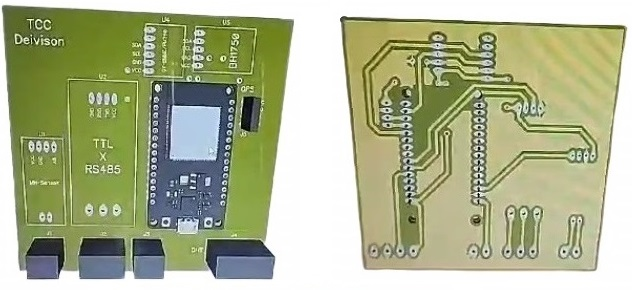
\includegraphics[width=16cm]{figuras/prototype-pcb.jpg}
    \fonte{Elaborado pelo autor, 2024.}
  \end{varwidth}
\end{figure}

\begin{figure}[!htb] \centering
  \caption{Matriz exportada do EasyEDA} \label{figura:pcb-scheme}
  \begin{varwidth}{\linewidth}
    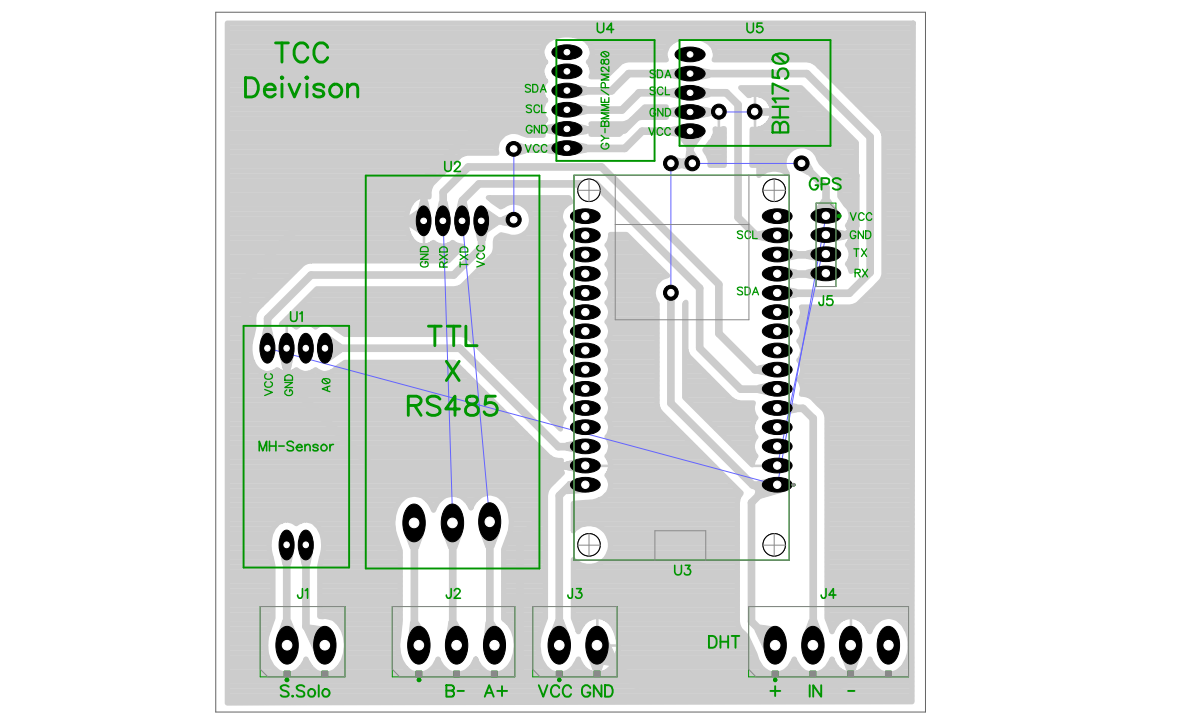
\includegraphics[width=16cm]{figuras/pcb-scheme.png}
    \fonte{Elaborado pelo autor, 2024.}
  \end{varwidth}
\end{figure}

\begin{figure}[!htb] \centering
  \caption{Matriz impressa em papel-filme} \label{figura:pcb-matriz}
  \begin{varwidth}{\linewidth}
    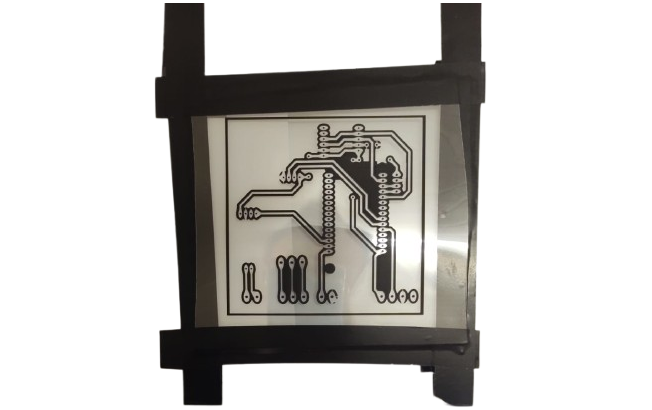
\includegraphics[width=16cm]{figuras/pcb-matriz.png}
    \fonte{Elaborado pelo autor, 2024.}
  \end{varwidth}
\end{figure}

\newpage

\begin{figure}[!htb] \centering
  \caption{PCB finalizada} \label{figura:pcb-pos}
  \begin{varwidth}{\linewidth}
    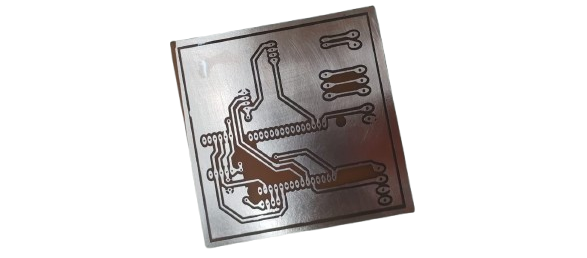
\includegraphics[width=16cm]{figuras/pcb-pos.png}
    \fonte{Elaborado pelo autor, 2024.}
  \end{varwidth}
\end{figure}

\begin{figure}[!htb] \centering
  \caption{PCB pós-corrosão} \label{figura:pcb-stg1}
  \begin{varwidth}{\linewidth}
    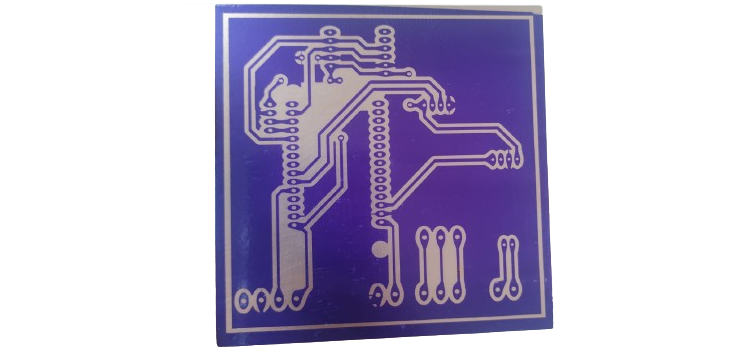
\includegraphics[width=16cm]{figuras/pcb-stg1.png}
    \fonte{Elaborado pelo autor, 2024.}
  \end{varwidth}
\end{figure}

\newpage

Para a prototipagem do \textit{software}, foram utilizados \textit{mockups} e \textit{wireframes} para definir as interfaces e fluxos de usuário. Ferramentas como \textit{Figma} foram empregadas para criar protótipos das telas, que serviram de guia para o desenvolvimento do \textit{frontend} em \textit{Next.js}. A distribuição dos componentes de \textit{software} seguiu o princípio de modularidade, permitindo que cada módulo fosse desenvolvido e testado isoladamente antes de ser integrado ao sistema principal.

A metodologia adotada permitiu uma transição suave do protótipo para a implementação final, garantindo que todos os componentes do sistema fossem adequadamente validados e integrados antes da implantação no laboratório.

\chapter{Resultados}

Nesta seção, são apresentados os resultados obtidos com o sistema desenvolvido, incluindo capturas das interfaces e do \textit{hardware} implementado. Também são apresentados gráficos dos dados coletados e armazenados pela aplicação, nomeada de \textit{IrrigaSync}.

\section{Interfaces do sistema \textit{IrrigaSync}}

Nas Figuras \ref{figura:irrigaDesktop} e \ref{figura:irrigaMobile}, são apresentadas imagens da interface do sistema \textit{IrrigaSync} em dispositivos \textit{desktop} e móveis, respectivamente, já na versão final de lançamento (\textit{release branch}).

\begin{figure}[!htb] \centering
\caption{\textit{IrrigaSync desktop}} \label{figura:irrigaDesktop}
\begin{varwidth}{\linewidth}
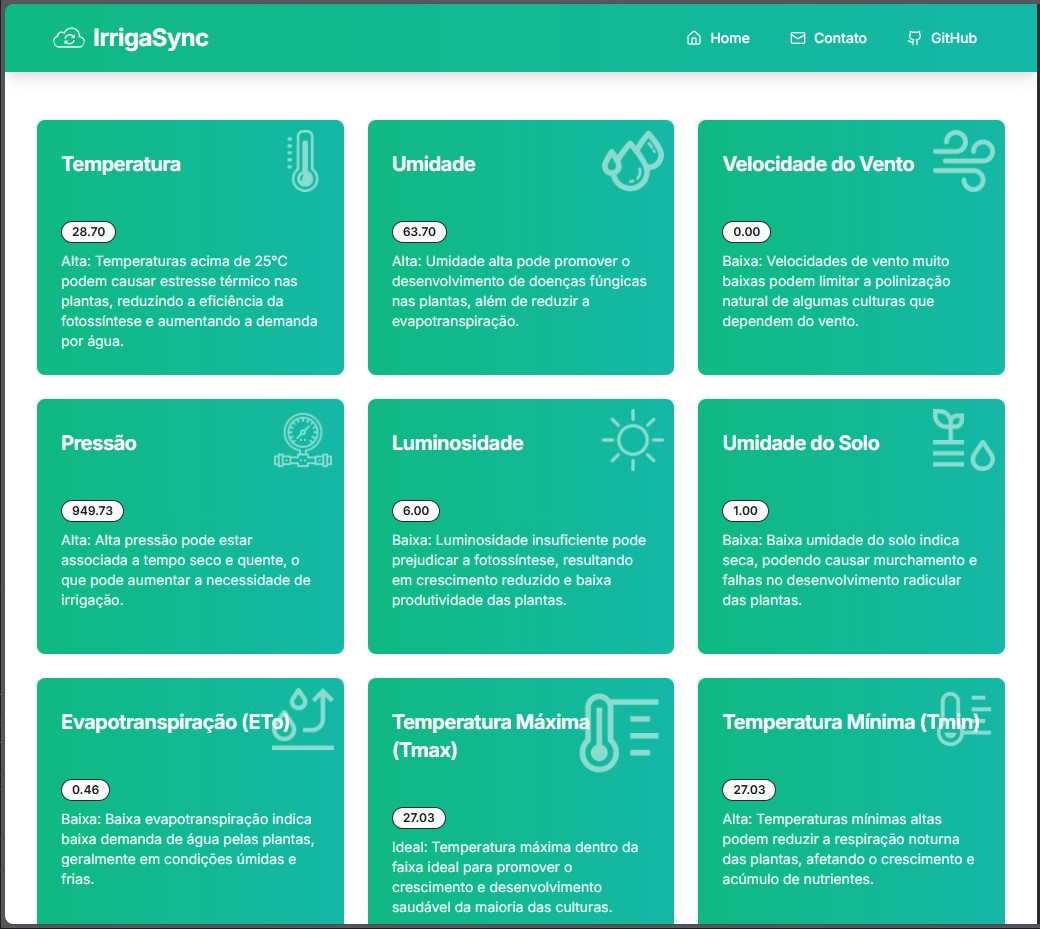
\includegraphics[width=16cm]{figuras/irrigaSync.png}
\fonte{Elaborado pelo autor, 2024.}
\end{varwidth}
\end{figure}

\begin{figure}[!htb] \centering
\caption{\textit{IrrigaSync mobile}} \label{figura:irrigaMobile}
\begin{varwidth}{\linewidth}
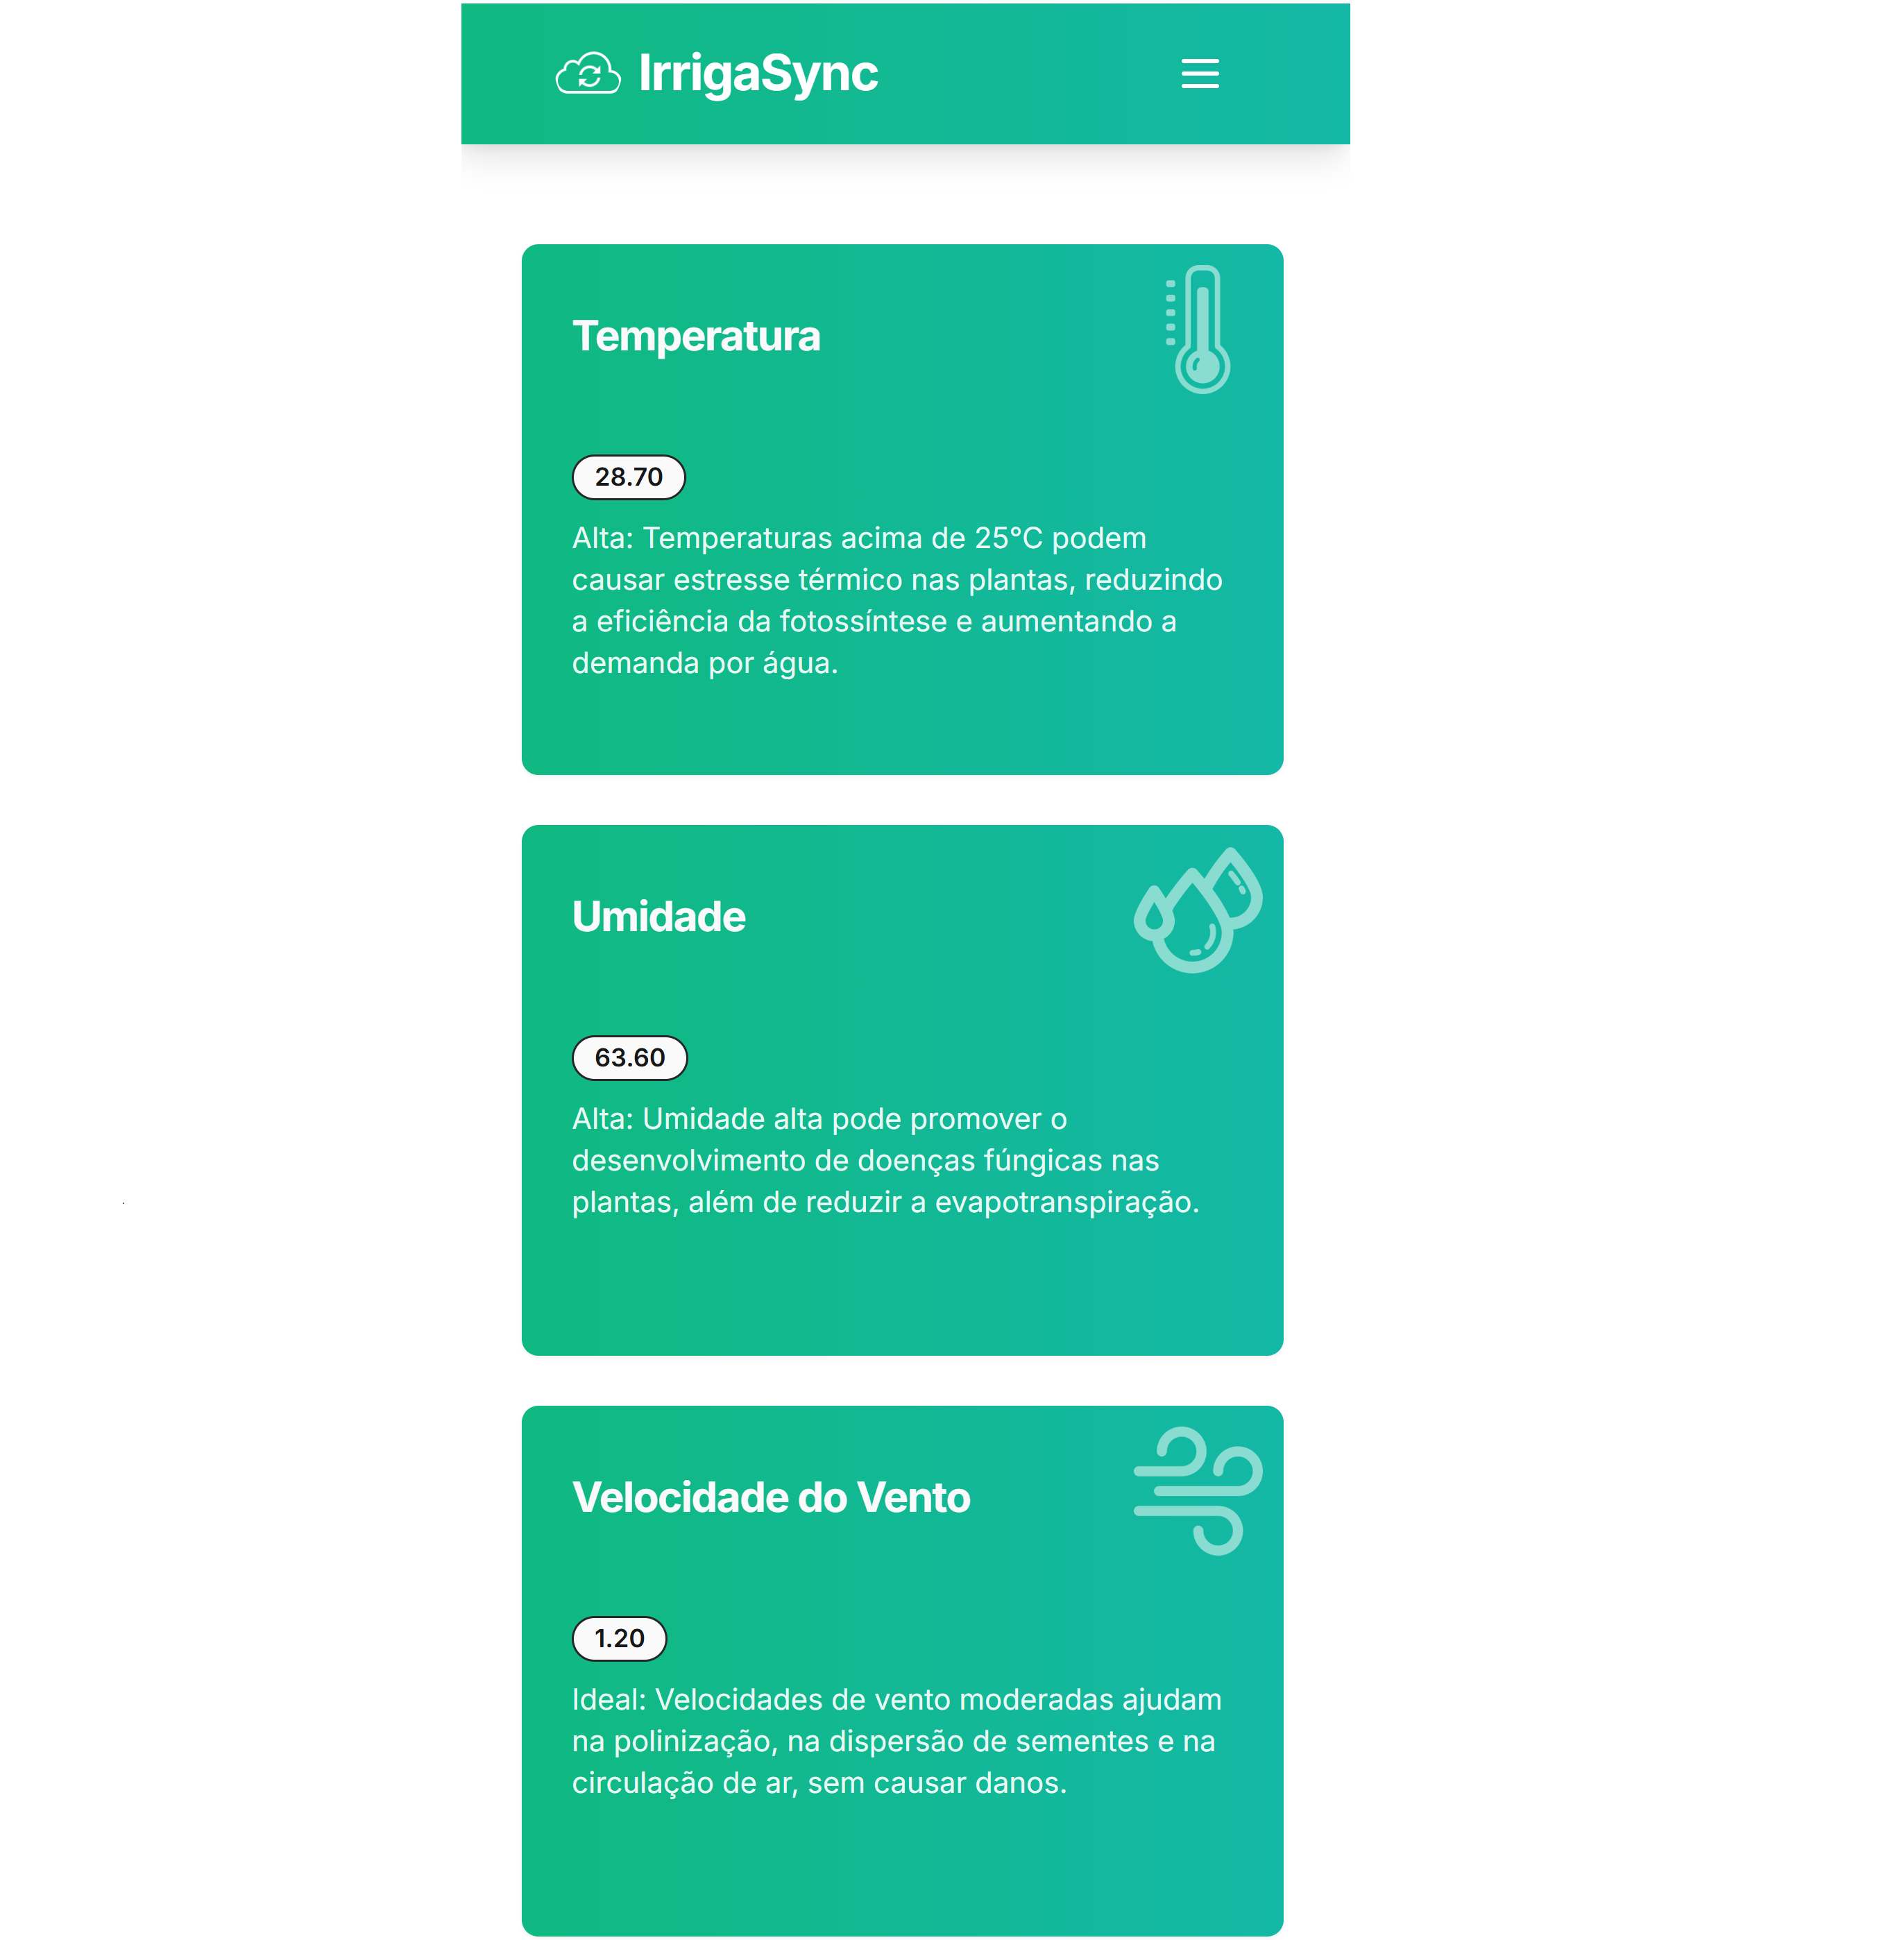
\includegraphics[width=16cm]{figuras/irrigaSyncMobile.png}
\fonte{Elaborado pelo autor, 2024.}
\end{varwidth}
\end{figure}

\section{Montagem do \textit{hardware}}

Para ilustrar o processo de montagem do \textit{hardware}, a Figura \ref{figura:gab-proj} apresenta o gabinete contendo a PCB instalada e os componentes integrados. Essa montagem final foi projetada para oferecer proteção contra intempéries e garantir a estabilidade do sistema.

\begin{figure}[!htb] \centering
\caption{Gabinete com PCB instalado} \label{figura:gab-proj}
\begin{varwidth}{\linewidth}
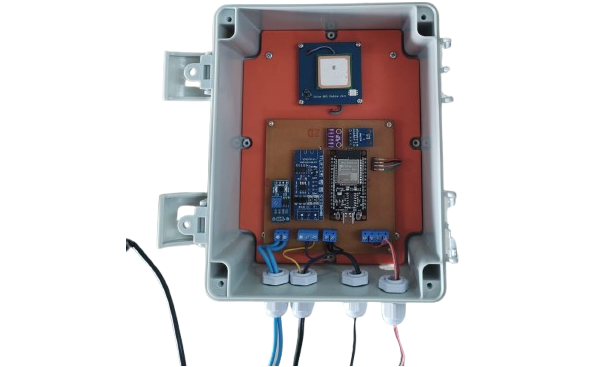
\includegraphics[width=16cm]{figuras/gab-proj.png}
\fonte{Elaborado pelo autor, 2024.}
\end{varwidth}
\end{figure}

\section{Dados coletados}

Os dados meteorológicos capturados diretamente pelo sistema incluem temperatura, umidade relativa do ar, velocidade do vento, luminosidade e pressão atmosférica. A seguir, estão as descrições dos principais resultados obtidos para cada variável durante um dia no local de implementação (16/10/2024).

\subsection{Temperatura e umidade relativa do ar}
Os valores de temperatura e umidade relativa foram obtidos a partir do sensor DHT22. A temperatura variou entre 19\textdegree C e 30\textdegree C, enquanto a umidade relativa oscilou entre 40\% e 85\%. Os gráficos da Figura \ref{fig:leituras-temp} e Figura \ref{fig:leituras-umid} apresentam a evolução desses parâmetros ao longo de um período de 12 horas.

\begin{figure}[!htb] \centering
  \caption{Evolução da temperatura em 12 horas (06:00 - 18:00)} \label{fig:leituras-temp}
  \begin{varwidth}{\linewidth}
    \includegraphics[width=16cm]{figuras/Temperatura_°C.png}
    \fonte{Elaborado pelo autor, 2024.}
  \end{varwidth}
\end{figure}

\begin{figure}[!htb] \centering
  \caption{Evolução da umidade em 12 horas (06:00 - 18:00)} \label{fig:leituras-umid}
  \begin{varwidth}{\linewidth}
    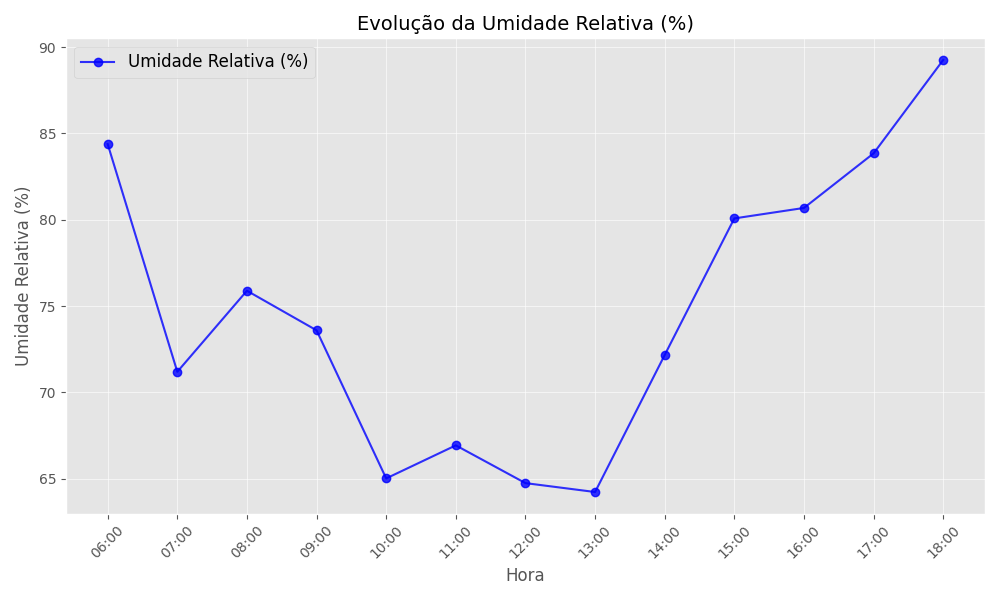
\includegraphics[width=16cm]{figuras/Umidade_Relativa.png}
    \fonte{Elaborado pelo autor, 2024.}
  \end{varwidth}
\end{figure}

\subsection{Velocidade do vento}
As medições de velocidade do vento, capturadas pelo anemômetro RS-FSJT-N01, mostraram uma variação entre 0.5 m/s e 12 m/s. A Figura \ref{fig:leituras-vel} ilustra a distribuição das velocidades ao longo de 12 horas.

\begin{figure}[!htb] \centering
  \caption{Evolução da velocidade do vento em 12 horas (06:00 - 18:00)} \label{fig:leituras-vel}
  \begin{varwidth}{\linewidth}
    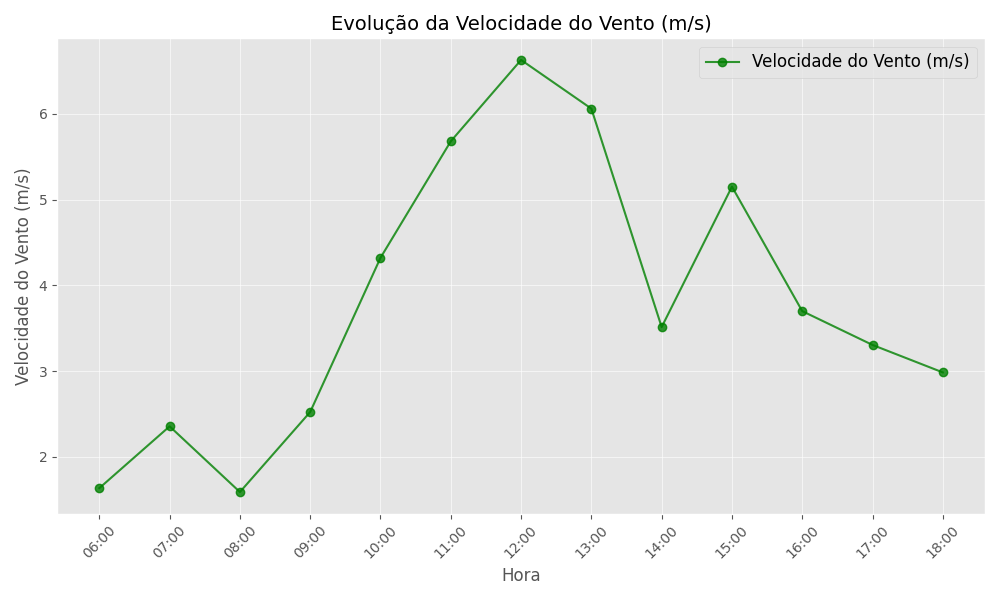
\includegraphics[width=16cm]{figuras/Velocidade_do_Vento_m_s.png}
    \fonte{Elaborado pelo autor, 2024.}
  \end{varwidth}
\end{figure}

\subsection{Luminosidade}
A intensidade luminosa medida pelo sensor BH1750 variou entre 400 lux e 25000 lux, refletindo mudanças na radiação solar ao longo do dia. A Figura \ref{fig:leituras-lum} mostra a evolução da luminosidade em função do tempo.

\begin{figure}[!htb] \centering
  \caption{Evolução da luminosidade em 12 horas (06:00 - 18:00)} \label{fig:leituras-lum}
  \begin{varwidth}{\linewidth}
    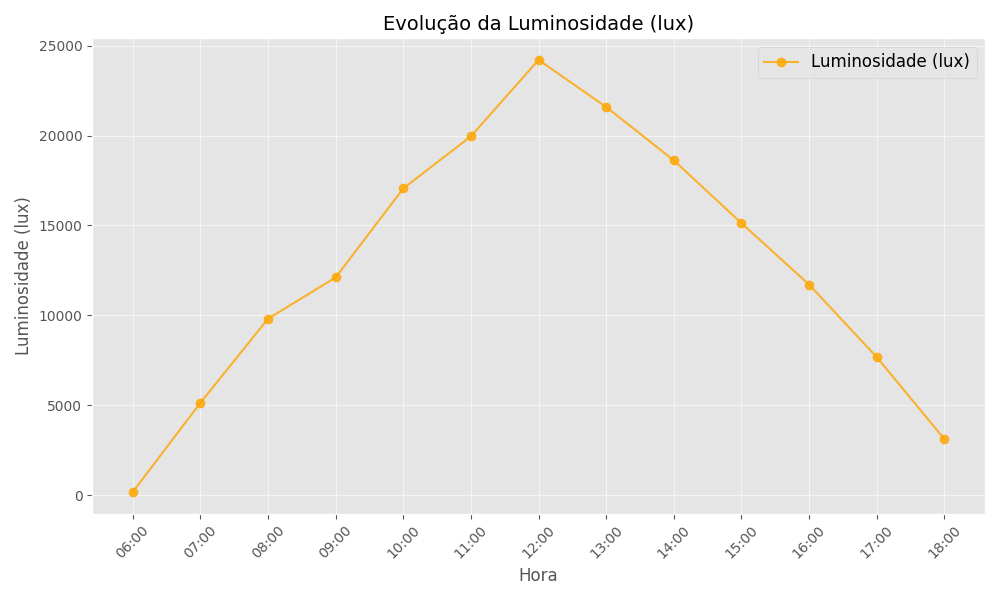
\includegraphics[width=16cm]{figuras/Luminosidade_lux.png}
    \fonte{Elaborado pelo autor, 2024.}
  \end{varwidth}
\end{figure}

\subsection{Pressão atmosférica}
O sensor BMP280 registrou valores de pressão atmosférica entre 950 hPa e 1020 hPa, refletindo as variações da região de Bambuí. A evolução da pressão ao longo do tempo é mostrada na Figura \ref{fig:leituras-pres}.

\begin{figure}[!htb] \centering
    \caption{Evolução das variáveis meteorológicas ao longo de 12 horas (06:00 - 18:00)} \label{fig:leituras-pres}
    \begin{varwidth}{\linewidth}
      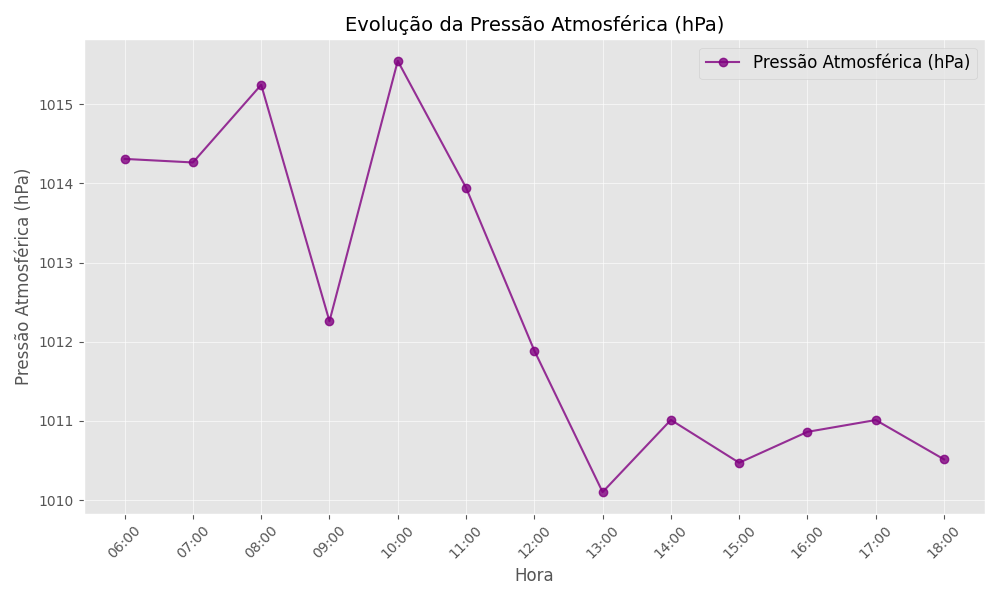
\includegraphics[width=16cm]{figuras/Pressão_Atmosférica_hPa.png}
      \fonte{Elaborado pelo autor, 2024.}
    \end{varwidth}
\end{figure}

\section{Comparação com dados de referência}

Para comparar os dados coletados pelo sistema \textit{IrrigaSync} em 16/10/2024, foram utilizadas informações do \textcite{inmet2024}, cuja estação climática se encontra no IFMG, \textit{Campus} Bambuí. A Tabela \ref{tab:comparacao-dados} apresenta uma comparação entre as variáveis climáticas registradas pelo \textit{IrrigaSync} e os dados disponíveis do INMET para a mesma data, período e horário.

\begin{table}[!htb] 
  \caption{Comparação dos dados climáticos em Bambuí em 16/10/2024} 
  \label{tab:comparacao-dados} 
  \begin{tabularx}{\textwidth}{|X|X|X|} \hline 
      \textbf{Variável} & \textbf{\textit{IrrigaSync}} & \textbf{INMET} \\ \hline 
      Temperatura Mínima (\textdegree C) & 19 & 20 \\ \hline 
      Temperatura Máxima (\textdegree C) & 33 & 38 \\ \hline 
      Umidade Relativa Mínima (\%) & 65 & 40 \\ \hline 
      Umidade Relativa Máxima (\%) & 85 & 80 \\ \hline 
  \end{tabularx}
  \fonte{Dados do sistema \textit{IrrigaSync} e do \textcite{inmet2024}.}
\end{table}

Observa-se que os dados de temperatura mínima e umidade relativa máxima registrados pelo \textit{IrrigaSync} estão próximos aos valores fornecidos pelo INMET. No entanto, há uma discrepância na temperatura máxima e na umidade relativa mínima. Essa diferença pode ser atribuída a fatores como a localização específica dos sensores do \textit{IrrigaSync}, possíveis microclimas locais ou variações nos horários de medição.

É importante considerar que os dados do INMET são obtidos de estações meteorológicas padronizadas e calibradas regularmente, enquanto o \textit{IrrigaSync} é um sistema em desenvolvimento que pode necessitar de ajustes e calibrações adicionais para melhorar a precisão de suas medições.

\section{Estimativa da evapotranspiração}

Com base nas variáveis coletadas, o sistema calculou a ETo e a ETc para uma pequena plantação de café arábica utilizando o método FAO-56 \parencite{Allen_evapotranspiration1998}. A plantação, situada ao lado do laboratório, corresponde a uma microcultura, cobrindo uma área de aproximadamente 6260,5 m², com condições controladas e específicas (Figura \ref{fig:plantacao-cafe}).

\begin{figure}[!htb] \centering
  \caption{Microcultura de café arábica do IFMG - \textit{Campus} Bambuí} \label{fig:plantacao-cafe}
  \begin{varwidth}{\linewidth}
    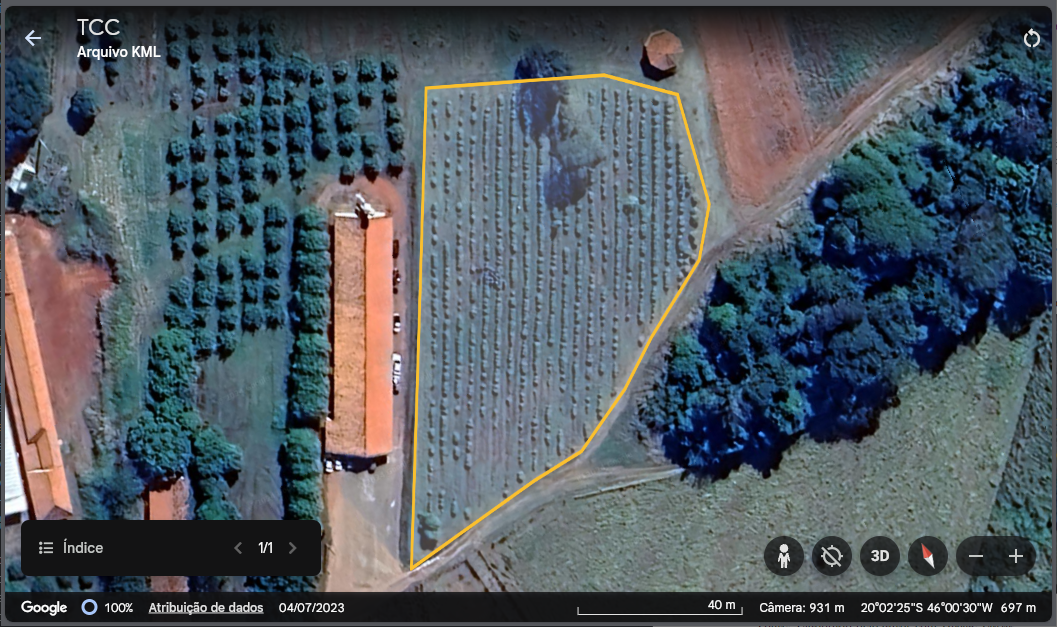
\includegraphics[width=16cm]{figuras/plantacao-cafe.png}
    \fonte{Elaborado pelo autor com \textit{Google Earth}.}
  \end{varwidth}
\end{figure}

De acordo com \textcite{rodrigues2013}, o Kc do café arábica varia de acordo com o estágio de desenvolvimento da planta e o manejo de irrigação. Em lavouras irrigadas, o valor do Kc para o café arábica pode variar ao longo do ano entre 0,21 e 0,80, com uma média de 0,57, dependendo das condições e do manejo da cultura.
No caso específico para essa época do ano, em outubro, geralmente, há uma variação dependendo da fase fenológica da planta e das condições climáticas da região. 

Estudos mostram que valores de Kc entre 0,72 e 1,50 são comuns em períodos de maior demanda hídrica, que ocorrem tipicamente entre junho e setembro, mas isso pode se estender, especialmente se houver alta evapotranspiração \parencite{souza2005}. Esses valores podem ser ajustados conforme o manejo de irrigação local, como observado em estudos feitos em Minas Gerais, onde o clima e a metodologia de irrigação impactam bastante o valor do Kc aplicado.

Para adotar um valor médio confiável do Kc para o café arábica utilizando uma abordagem científica, um valor de 0,60 é, geralmente, uma boa referência durante o ano, especialmente em lavouras irrigadas \parencite{rodrigues2013}. Isso é corroborado por estudos que mostram que o Kc do café arábica varia entre 0,21 e 0,80, com um valor médio ao longo do ciclo produtivo próximo a 0,57. No sistema implementado, o valor de Kc pode ser definido como entrada ao clicar na logo da aplicação na barra de navegação superior, sendo que, para a microcultura em questão, foi adotado o valor de 0,60.

A Tabela \ref{tab:et} apresenta os valores estimados para ETo e ETc no dia 16/10/2024, para essa microcultura de café arábica, capturados pelo sistema \textit{IrrigaSync}.

\begin{table}[!htb]
  \caption{Valores de ETo e ETc coletados pelo sistema \textit{IrrigaSync}} \label{tab:et}
  \begin{tabularx}{\textwidth}{|c|X|X|} \hline
    \textbf{Hora} & \textbf{ETo (mm/dia)} & \textbf{ETc (mm/dia)} \\ \hline
    06:00 & 2.88 & 1.73 \\ \hline
    09:00 & 4.32 & 2.59 \\ \hline
    12:00 & 6.00 & 3.60 \\ \hline
    15:00 & 4.80 & 2.88 \\ \hline
    18:00 & 3.60 & 2.16 \\ \hline
  \end{tabularx}
  \fonte{Resultados obtidos do sistema \textit{IrrigaSync}.}
\end{table}

A escolha do café arábica como cultura monitorada reflete a relevância da sua produção na região. Os dados obtidos podem ser úteis para o manejo preciso de água e o controle climático dessa microcultura, exemplificando a aplicabilidade do sistema \textit{IrrigaSync}.

\section{Discussão dos resultados}

Os resultados apresentados demonstram o funcionamento do sistema \textit{IrrigaSync} para monitoramento ambiental e suporte ao manejo de irrigação em uma microcultura de café arábica. A integração entre o \textit{hardware} e o \textit{software} garantiu a coleta e o processamento de dados relevantes para o contexto agrícola, permitindo a estimativa da evapotranspiração.

A análise dos dados coletados revelou que, embora o sistema atenda aos requisitos funcionais propostos, algumas limitações precisam ser abordadas para garantir maior precisão e confiabilidade. Por exemplo, a comparação com os dados do INMET mostrou discrepâncias em algumas variáveis, como a temperatura máxima e a umidade relativa mínima. Tais diferenças podem ser atribuídas a fatores como localização dos sensores, presença de microclimas locais e calibração inicial dos equipamentos.  

Além disso, a análise da infraestrutura revelou desafios relacionados à cobertura da rede \textit{Wi-Fi} no laboratório, o que limitou a transmissão de dados em tempo real em algumas áreas. 

O sistema também apresentou limitações no sensor de umidade do solo, que registrou variações mais amplas do que o esperado. Isso sugere a necessidade de uma análise mais rigorosa do desempenho desse sensor, incluindo possíveis substituições por modelos mais precisos e adequados ao ambiente em questão.  

Outro ponto relevante é a aplicabilidade do \textit{IrrigaSync} para diferentes culturas agrícolas. Embora o protótipo tenha sido validado em uma microcultura de café arábica, sua modularidade e flexibilidade permitem adaptações para outros tipos de cultivo. No entanto, para garantir a eficácia em diferentes cenários, ajustes nos valores de \textit{Kc} são necessários, considerando fatores específicos de cada cultura.  



\chapter{Conclusão}

A realização deste trabalho apresentou um sistema  para monitoramento agrícola em tempo real, abordando as necessidades específicas de manejo hídrico e climático para culturas agrícolas. O desenvolvimento da solução baseou-se em boas práticas de engenharia de \textit{software} e \textit{hardware}, garantindo uma integração consistente entre os componentes físicos e computacionais. Além disso, o sistema permitiu a coleta de dados ambientais relevantes, como temperatura, umidade, radiação solar, pressão atmosférica e velocidade do vento, utilizados para calcular a evapotranspiração (ETo e ETc) com base no método FAO-56 \parencite{Allen_evapotranspiration1998}.

Os resultados obtidos demonstraram que o sistema atende aos objetivos propostos, especialmente no que tange à usabilidade, flexibilidade e capacidade de adaptação a diferentes cenários agrícolas. A interface intuitiva contribuiu para a acessibilidade e compreensão dos dados pelos usuários finais, enquanto a modularidade da solução oferece espaço para melhorias e expansões futuras.

Contudo, algumas limitações foram identificadas, como a necessidade de calibração mais frequente do sensor de umidade do solo e a dependência de conectividade \textit{Wi-Fi} no raio de acesso. Apesar dessas questões, o sistema mostrou-se promissor e funcional dentro das condições de teste na microcultura observada, com potencial para aplicação em escalas maiores.

Em suma, este trabalho apresenta uma contribuição para o manejo sustentável da agricultura, ao propor uma ferramenta prática e acessível que alia tecnologia e ciência no auxílio à tomada de decisões em campo. As perspectivas de evolução do sistema, descritas na próxima seção, reforçam a viabilidade de ampliação do impacto deste projeto para diferentes cenários e culturas agrícolas.

\chapter{Trabalhos futuros}

O sistema \textit{IrrigaSync} oferece uma base para desenvolvimento contínuo e melhorias. Algumas direções futuras incluem:  

\begin{enumerate}
    \item Otimização do sistema
        \begin{itemize}
            \item Melhorar os algoritmos de cálculo da evapotranspiração, incorporando novos métodos e equações adaptadas a diferentes condições climáticas e culturas específicas.  
            \item Desenvolver rotinas de autoavaliação para o sistema, permitindo diagnósticos automatizados de falhas em sensores e componentes de rede.  
        \end{itemize}
    \item Calibração e validação
        \begin{itemize}
            \item Realizar calibrações periódicas mais detalhadas para reduzir discrepâncias nos dados coletados, especialmente em relação a fontes oficiais, como o INMET e de outros sistemas de referência. 
            \item Investigar as influências de microclimas locais de forma mais sistemática, para adequar o sistema a diferentes cenários geográficos.  
        \end{itemize}
    \item Expansão funcional  
        \begin{itemize}
            \item Integrar sensores adicionais, como medidores de qualidade do ar e sensores de nutrientes para análise do solo.  
            \item Incorporar funcionalidades preditivas, utilizando algoritmos de aprendizado de máquina, para prever demandas hídricas e riscos climáticos.  
        \end{itemize}
    \item Interoperabilidade e automação  
        \begin{itemize}
            \item Explorar a integração com sistemas de irrigação automatizados, permitindo controle dinâmico baseado em dados em tempo real.  
            \item Desenvolver conectores para plataformas agrícolas existentes e para dispositivos inteligentes, como assistentes virtuais e \textit{smart hubs}.  
        \end{itemize}
    \item Acessibilidade e escalabilidade
        \begin{itemize}
            \item Ampliar a cobertura do sistema em áreas com conectividade limitada, utilizando redes LoRa, Sigfox ou sistemas híbridos.  
            \item Adaptar o sistema para culturas agrícolas de maior escala, analisando seu desempenho em condições de larga produção.  
        \end{itemize}
    \item Validação científica e industrial  
        \begin{itemize}
            \item Promover estudos de caso com diferentes tipos de cultivo, em parceria com produtores rurais e instituições de pesquisa, para avaliar o impacto do sistema na produtividade e sustentabilidade agrícola.  
            \item Buscar certificações e validações que permitam a utilização comercial do sistema em larga escala.  
        \end{itemize}
\end{enumerate}

Essas melhorias e expansões podem consolidar o \textit{IrrigaSync} como uma solução de referência para monitoramento agrícola, contribuindo para uma agricultura mais sustentável, eficiente e tecnológica.


%\chapter{Modelos de referências}

%\input{capitulos/cap_modelos_referencias}

% -------------------------------------------------------
% Elementos pós-textuais
% -------------------------------------------------------
\postextual

% -------------------------------------------------------
% Referências bibliográficas
% -------------------------------------------------------

\printbibliography
% Na prática pode ser usado apenas \printbibliography
% O comando \printbibliography[notkeyword=exemplo] foi usado para não mostrar as referências do capítulo de exemplo
% -------------------------------------------------------
% Apêndices
% -------------------------------------------------------
%\apendices

%\partapendices

%\chapter{Documento básico usando a classe {IF\TeX}}

%\input{capitulos/apendice_doc_basico_if}

% -------------------------------------------------------
% Anexos
% -------------------------------------------------------
%\anexos

%\partanexos

%\chapter{Páginas interessantes na internet} \label{capitulo:paginas_interessantes}

%\input{capitulos/anexo_paginas_interessantes}

\end{document}